% !TEX root = ../notes_template.tex
\chapter{Population Movement and Habitat Selection}\label{Chap10_movement}

\section{From Individual to Population Movement} \label{sec:Chap10_Eulerian_movement}

In Chapter \ref{sec:Chap4_movement}, we introduced the general importance of movement within ecological theory and applications.  We then demonstrated how to fit a model for individual movement from a Lagrangian viewpoint, which tracks changes in the location \(S_{i}(t)\) for one or more individuals \(i\) at each time \(t\).  We specifically solved functions describing dynamics using an Euler approximation that discretized continuous time into time-intervals with spacing \(\Delta_t\) while tracking individual location \(S_{i,t}\) in continuous space.  We then decomposed movement over each interval into \textit{taxis} (i.e., movement toward preferred habitats), \textit{drift} (i.e., directional movement), and \textit{diffusion} (i.e., otherwise unexplained movement) (see definitions in Section \ref{sec:Chap4_movement_ecology}).  We showed that we could model individual movement in this continuous-space and discrete-time framework by treating location as a random effect in a multivariate state-space model, and that we could model movement for multiple animals by expanding the set of state-space variables.  We then showed that this had many practical advantages, e.g.:
\begin{enumerate}
    \item The model can be used both to simulate dynamics and data resulting from individual movement, or efficiently fitted to those same data to estimate unknown movement parameters;
    
    \item We could specify a preference function \(h(s)\) and apply the \textit{gradient operator} to this function \(\nabla h(s)\), which results in a vector that points in the direction of increasing habitat preference.  Individuals are then expected to move in the direction of this vector, i.e., toward preferred habitats (Eq. \ref{eq:Chap4_differential_equation});

    \item A fitted model can be used to predict animal location at times between sequential measurements.  Predictive variance was then lowest when location was measured and was higher during times between measurements;

    \item The model could be fitted simultaneously to data from multiple individuals, and movement that is correlated among individuals can be approximated by assembling the covariance among individuals using techniques derived from factor-analysis or structural equation models.
\end{enumerate}
However, fitting a movement process as a state-space model from a Langrangian viewpoint becomes computationally expensive (or prohibitive) as the number of individuals increases.  

To overcome computational limits when dealing with dynamics involving movement of many individuals, we now change from the Lagrangian (individual-based) to Eulerian (grid-based) viewpoint. We specifically track animal densities \(d(s,t)\) across continuous space \(s\) and continuous time \(t\), while still describing movement resulting from the same combination of taxis, drift, and diffusion.  This can be written compactly as a partial differential equation (see Table \ref{tab:Appendix_expression} for a summary of notation):  

\begin{equation} \label{eq:Chap10_PDE}
    \frac{\partial}{\partial t} d(s,t) = 
    \underbrace{D \nabla^2 d(s,t)}_{\mathrm{diffusion}}
    - \underbrace{\mathbf{v}(s) \cdot \nabla d(s,t)}_{\mathrm{drift}} 
    - \underbrace{\nabla h(s) \cdot \nabla d(s,t)}_{\mathrm{taxis}}   
\end{equation}
where \(\mathbf{v}(s)\) is a vector representing the direction of drift, \(\nabla d(s,t)\) is the gradient of the density function, \(\nabla h(s)\) is the gradient of the preference function (defined identically to Eq. \ref{eq:Chap4_differential_equation}), \( \nabla^2 d(s,t) \) is the \myindex{Laplace operator} for the density function which is computed as the second derivative of density function \(d(t)\) evaluated at \(s\), and \(D = \frac{\sigma^2}{2}\) is the diffusion coefficient where \(\sigma^2\) is the variance in displacement that occurs per unit time from diffusion alone.  We doubt that many ecologists will be familiar with this partial differential equation (PDE) notation, so we briefly summarize the components here:

\begin{itemize}
    \item \textit{Drift}:  \(\mathbf{v}(s) \cdot \nabla d(s,t)\) is the dot product of the vector \(\mathbf{v}(s)\) that points in the direction of passive drift and the vector \(\nabla d(s,t)\) that points toward higher densities.  This dot product is positive if densities are increasing in the same direction as drift is pushing animals, and this will result in a local decrease in densities over time as the lower density of animals upstream is then advected to replace the animals currently at location \(s\).  Similarly, if the drift vector is pointing in one direction (e.g., north), and the vector of increasing density is orthogonal (e.g., east), then the dot product is zero.  Passive drift will have no effect on local densities in this case because each packet of individuals that is advected northward is replaced by a packet of individuals with similar density;

    \item \textit{Taxis}: \(\nabla h(s) \cdot \nabla d(s,t)\) is the dot product of the gradient of the preference function and the gradient of the density function.  This will be positive if animal densities are increasing in the same direction as the increase in preference, which will again cause local densities to decrease;  

    \item \textit{Diffusion}:  \(\nabla^2 d(s,t)\) is the Laplacian of the density function, calculated by taking the matrix of second derivatives of the density function at \(s\) and calculating the sum of diagonal entries (the trace of the Hessian matrix).  This measures the curvature of the density function at location \(s\); if \(d(t)\) curves downward (i.e., \(\nabla^2 d(s,t)\) is negative) then emigration exceeds immigration and diffusion causes local densities to decrease, while if it is positive then diffusion causes local densities to increase.  To see this, imagine the case involving a single spatial dimension.  If density function \(d(t)\) has a local maximum at location \(s\), then the second derivative is by definition negative.  This will then result in a decrease in local densities as animals emigrate from that local maximum faster than immigration from nearby locations with lower densities. Similarly, if the second derivative is positive in this one-dimensional example, then densities will tend to increase from diffusion as immigration exceeds emigration to nearby locations.   
\end{itemize}
Both taxis and drift represent different types of advective movement, so we can call Eq. \ref{eq:Chap10_PDE} an advection-diffusion model. We previously referred to a random-walk process for location as diffusive movement, but note that the term diffusion refers specifically to a PDE (e.g., Eq. \ref{eq:Chap10_PDE}).

\section{General Solution for Movement Processes} \label{sec:Chap10_solving_movement_process}

This PDE representing movement (Eq. \ref{eq:Chap10_PDE}) can be solved analytically for some specific density and preference functions\footnote{See https://github.com/james-thorson/Spatio-temporal-models-for-ecologists/Chap\_10 for code associated with this chapter.}.  In fact, we used these solutions already in Section \ref{sec:Chap4_diffusion_and_taxis} to calculate the expected density function in time \(t+\Delta_t\) given a known location in time \(t\), which we used to define the multivariate normal distribution used to simulate movement (e.g., Eq. \ref{eq:Chap4_difference_equation}).  

For example, assuming that we know the location of an animal \(\mathbf{s}_0\) at some initial time \(t_0\) and that drift and taxis are absent, we can use Eq. \ref{eq:Chap4_diffusion} to compute a probability density for the animal being at any location \(\mathbf{s}\) after interval \(\Delta_t\) elapses:
\begin{equation} \label{eq:Chap10_diffusion_density}
    d(\mathbf{s},t_0+\Delta_t) = \mathrm{dMVN}( \mathbf{s}_0, \Delta_t \sigma^2 \mathbf{I} )
\end{equation}
We can then use this \textit{fundamental solution} to check how Eq. \ref{eq:Chap10_PDE} works in the known case (Code \ref{code:Chap10-analytical-solution}) of diffusive movement. To do so, we select a starting location, diffusion covariance \colorbox{backcolour}{Sigma}, and randomized location \colorbox{backcolour}{s0}  and time \colorbox{backcolour}{t0} to evaluate.  We then create a function \colorbox{backcolour}{Density} that computes the known density function at that time and place (Eq. \ref{eq:Chap10_diffusion_density}). Finally, we use package \colorbox{backcolour}{numDeriv} \cite{gilbert_numderiv_2019} to compute finite-difference approximations to this density function, which we use to compare the time-gradient for this function (i.e., the left-hand-side of Eq. \ref{eq:Chap10_PDE}) and the Laplacian operator (i.e., the right-hand-side of Eq. \ref{eq:Chap10_PDE}).  This confirms that Eq. \ref{eq:Chap10_PDE} holds numerically in this known case.  

\lstset{style=Rcode}
\lstinputlisting[language=R, firstline=4, lastline=22, label=code:Chap10-analytical-solution, caption=R code for analytical solution to partial differential equation for diffusion., captionpos=t]{Chap_10/PDE_example.R} 

However, we instead seek to solve the movement PDE generically for a wide range of ecological contexts.  To do so, we discretize the model by switching to an Eulerian viewpoint (see Section \ref{sec:Chap1_IBMs} for discussion).  This proceeds via the following steps:
\begin{enumerate}
    \item \textit{Discretize space}: partitioning a spatial domain \( \mathcal{D} \) into a set of \( n_j \) non-overlapping spatial cells, such that we can approximate densities as being constant within each cell; 
    
    \item \textit{Define adjacency}:  defining an adjacency matrix \(\mathbf A\) with dimension \( n_j \times n_j \), having a value of one for any two cells that share an edge and zero otherwise;

    \item \textit{Define abundance matrix}: replacing the population density function \(d(s,t)\) from Eq. \ref{eq:Chap10_PDE} with an abundance matrix \(\mathbf{N}\) recording the number of individuals \( n_{j,t} \) in each grid cell \(s\) in time \(t\).  For a single organism, we can define this abundance vector as an indicator where \( n_{j,t} = 1 \) for the cell \(j\) where it resides at time \(t\) and zero elsewhere;

    \item \textit{Define movement matrix}: representing movement probabilities over a time-interval from \(t\) to \(t+\Delta_t\) via a movement matrix \(\mathbf{M}_t\) with dimension \( n_j \times n_j \);

    \item \textit{Project abundance via movement matrix}: calculating expected abundance \(\hat{\mathbf{n}}_{t+\Delta_t}\) after interval \(\Delta_t\) has elapsed as:
\begin{equation} \label{eq:Chap10_movement_projector}
   \hat{\mathbf{n}}_{t+\Delta_t}^T = \mathbf{n}_t^T \mathbf{M}_t 
\end{equation}
\end{enumerate}
These steps calculate the expected abundance following the movement processes represented by \(\mathbf{A}\), which we will construct to represent drift, taxis, and diffusion.  However, these steps do not include the variance resulting from individual stochasticity (i.e., the directed random walk followed by each individual in Eq. \ref{eq:Chap4_difference_equation}).  To see this, imagine that we use an indicator vector for density \(\mathbf{n}_t\), i.e., a vector of zeros except for a single 1, representing the spatial cell where a single organism resides in time \(t\).  This indicator matrix is multiplied by \(\mathbf{M}\), which results in a density \( 0 \leq d_j \leq 1 \) that is spread among multiple cells in time \(t+\Delta_t\).  However, a single individual does not itself diffuse.  Instead, it will move to a single new location, with expectation predicted by Eq. \ref{eq:Chap10_movement_projector}.  To represent stochasticitiy, we can add another step to the algorithm:

\begin{enumerate}
    \item[6] \textit{Simulate stochasticity}: simulating random variation in movement (i.e., stochasticity) by drawing a vector of realized abundance from a multinomial distribution with expected counts \( \hat{\mathbf{n}}_{t+\Delta_t} \):
\begin{equation} \label{eq:Chap10_movement_stochasticity}
   \mathbf{n}_{t+\Delta_t} \sim \mathrm{Multinomial}( \hat{\mathbf{n}}_{t+\Delta_t} ) 
\end{equation}    
    where the multinomial movement probabilities are calculated by dividing \(\hat{\mathbf{n}}_{t+\Delta_t}^T\) by its sum.  When sample sizes are large, this multinomial distribution will converge on its expectation \( \mathbf{n}_{t+\Delta_t} =\approx \hat{\mathbf{n}}_{t+\Delta_t} \) such that stochasticity becomes unimportant for large groups of independent individuals.
\end{enumerate}
For simplicity of presentation, we will describe individual movement from an Eulerian viewpoint in two dimensions using square grid cells with equal size and sides of length \(\Delta_s\).  However, the same concepts can then be generalized with small changes to notation and code to more dimensions, other cell shapes (hexagons, triangles, etc.), or unequally sized cells.  

The focus of interference then becomes: how do we specify a movement matrix \(\mathbf{M}\) that provides a suitable discretization to Eq. \ref{eq:Chap10_PDE} using an Eulerian viewpoint (i.e., Step-4 above)?  Ideally, this matrix would have several properties:
\begin{enumerate}
    \item[A] \textit{Conservation of numbers}:  we seek a movement-probability matrix \(\mathbf{M}\) that represents only the effect of movement while conserving population size, such that a model can be combined with other components that represent size-transitions, survival, recruitment, and other demographics;

    \item[B] \textit{Habitat utilization as stationary distribution}:  we seek a matrix such that, if it is repeatedly applied to a vector of initial abundance \(\mathbf{n}_0\), then abundance will converge on a stationary distribution that represents their expected long-term or average habitat utilization;
    
    \item[C] \textit{Identical parameters using either Eulerian or Lagrangian viewpoint}:  additionally, we seek to develop \(\mathbf{M}\) in such a way that the same parameters can be used in a model using a Lagrangian viewpoint (e.g. Chap \ref{sec:Chap4_movement}) to generate (nearly) identical dynamics;  

    \item[D] \textit{Complicated dynamics using few parameters}:  similarly, we seek a method that can include covariates, allows a wide range of model complexity (i.e., few or many estimated parameters), and can mimic complex behaviors with a small number of parameters;
    
    \item[E] \textit{Computational efficiency}:  we seek a method for constructing \(\mathbf{M}\) that remains computationally efficient even with a fine spatial resolution, and can be run quickly enough to allow Bayesian or maximum likelihood inference about parameters;
    
    \item[F] \textit{Scale-free discretization}:  finally, we seek a model where the spatial scale and grid shape used during discretization has little effect on the estimated value of model parameters for a given data set; 

    \item[G] \textit{Subdivision in time}:  as a corollary of the preceding property, we seek a method where we can calculate the movement fractions arising for any subdivision of time, i.e., \(n_{t + x \Delta_t}\) where \(0 < x< 1\) is some fraction of the modeled time-step so that, e.g., we can project the likely path of movement between two modeled times \(t\) and \(t+\Delta_t\) after the model is fitted.  
    
\end{enumerate}
In this chapter, we first introduce the theory of \textit{continuous-time Markov Chains}, which can satisfy all of these desired criteria. We then discuss how to parameterize these to create a movement-probability matrix.  

\section{Assembling a Movement Probability Matrix} \label{sec:Chap10_assembling_movement_matrix}

We specifically proceed by calculating movement matrix \( \mathbf M \) by first assembling a matrix of instantaneous movement rates \( \dot{\mathbf{M}} \).  This movement-rate matrix represents the instantaneous rate at which individuals move from one cell \( g_1 \) to another \( g_2 \) per unit time.  This movement-rate matrix therefore defines the instantaneous movement rate:

\begin{equation} \label{eq:Chap10_CTMC}
    \frac{\partial}{\partial t} \mathbf{n}_t^T = \mathbf{n}_t^T \dot{\mathbf{M}} 
\end{equation}
We then seek to integrate the action of this movement-rate matrix over a time-interval \( \Delta_t \):  

\begin{equation}
    \mathbf{n}_{t+\Delta_t}^T = \int_t^{t+\Delta_t} \mathbf{n}_t^T \dot{\mathbf{M}}  \delta t
\end{equation}
This integral can be computed by an operation called the \myindex{matrix exponential}:

\begin{equation} \label{eq:Chap10_matrix_exponential}
\begin{gathered}
    \mathbf{M} = e^{\Delta_t \dot{\mathbf{M}}} \\
    \mathbf{n}_{t+\Delta_t}^T = \mathbf{n}_t^T \mathbf{M}  
\end{gathered}
\end{equation}
where this equation defines a \myindex{continuous-time Markov Chain} (CTMC)\cite{hanks_continuous-time_2015}, representing first-order Markov transition rates among each grid cell.  The computational methods for software implementing the matrix exponential are complicated.  However, we believe that Eq. \ref{eq:Chap10_matrix_exponential} will be conceptually familiar to ecologists, who are familiar with exponential population growth.  In that well-known case, integrating population growth rate \(r\) over time \(\Delta_t\) is solved by multiplying initial population size by \(e^{\Delta_t r}\). The matrix exponential is also available in both R and TMB so we think that a conceptual understanding is sufficient for most users (see Appendix \ref{sec:Appendix_matrix_exponential} for more details regarding implementation).  We note that there are many other avenues to integrate Eq. \ref{eq:Chap10_CTMC} or the original movement PDE (Eq. \ref{eq:Chap10_PDE}).  In the following, we emphasize the matrix exponential precisely because we believe that many ecologists are already comfortable with text and code that applies the (scalar) exponential function to integrate time-series dynamics, such that the matrix exponential is a small expansion of this existing ``minimal toolkit" for statistical ecology.   

Ecological intuition immediately provides several rules for constructing movement-rate \(\dot{\mathbf{M}}\): 
\begin{itemize}
    \item \textit{No teleportation}:  individuals can only move to an adjacent cell, i.e., where adjacency matrix \(\mathbf A\) is nonzero.  The movement-rate matrix \( \dot{\mathbf{M}} \) then has the same sparsity pattern as \(\mathbf A\); 

    \item \textit{Conservation of numbers}:  individuals do not appear or disappear solely from the action of movement.  Therefore, the rows of \(\dot{\mathbf{M}}\) must sum to zero;

    \item \textit{No negative abundance of animals}:  the number of individuals in a given cell must be non-negative.  To ensure that abundance after movement \(\mathbf{n}_t^T \mathbf{M}\) is non-negative for any possible initial abundance \(\mathbf{n}_t^T\) that is also non-negative, it is sufficient to construct \(\dot{\mathbf{M}}\) as a \myindex{Metzler matrix}, defined as a matrix with non-negative values in the off-diagonal.  
\end{itemize}
Given conditions 2 (conservation of numbers) and 3 (no negative abundance), we see that the diagonal elements of \(\dot{\mathbf{M}}\) must also be non-positive, with value equal to the negative-sum of values in that row.

We also note that the matrix exponential can also be approximated by dividing the time-interval \(\Delta_t\) into \(N\) sub-intervals, and then approximating movement as a linear rate over each sub-interval.  This \textit{Euler method} (see Code \ref{code:Chap10-euler-approximation}) results in the following approximation to the matrix exponential:

\begin{equation} \label{eq:Chap10_euler_approximation}
    \mathbf{M} \approx (\mathbf{I} + \frac{\Delta_t}{N}\dot{\mathbf{M}})^N
\end{equation}
The resulting Euler approximation to \(\mathbf{M}\) has sparsity structure of \( \mathbf{A}^N \).  Adjacency matrix \(\mathbf{A}\) in turn is nonzero only for neighbors, so the Euler approximation is nonzero for any two cells only if you can get from one to the other by crossing at most \(N\) edges.  This implies that the Euler approximation is essentially truncating movement beyond \(N\) cells per interval.   

\lstset{style=Rcode}
\lstinputlisting[language=R, label=code:Chap10-euler-approximation, caption=R code for Euler approximation to matrix exponential., captionpos=t]{Shared_functions/matexp.R} 

Code \ref{code:Chap10-euler-approximation} demonstrates a conceptually simple approach to solve this CMTC by exponentiating a sparse movement-rate matrix \(\dot{\mathbf{M}}\) to calculate movement fractions \(\mathbf{M}\), and we use the package \colorbox{backcolour}{expm} \cite{maechler_expm_2023} for efficient computation of the matrix exponential involving a sparse matrix.  We therefore turn to discussing how to form the movement-rate matrix \(\dot{\mathbf{M}}\).  In particular, we decompose the movement-rate matrix into three additive components:  diffusion \(\dot{\mathbf{D}}\), taxis \(\dot{\mathbf{Z}}\), and passive advection \(\dot{\mathbf{V}}\) (recalling definitions in Section \ref{sec:Chap4_movement_ecology}):

\begin{equation}
    \dot{\mathbf{M}} = \dot{\mathbf{D}} + \dot{\mathbf{Z}} + \dot{\mathbf{V}}    
\end{equation}
where these components are all matrices with the same sparsity pattern as \(\mathbf A\), such that \(\dot{\mathbf{M}}\) also has this sparsity pattern.  Each component then represents different mechanistic assumptions about dominant movement processes.  

Similar to our movement models from a Lagrangian viewpoint, diffusion again represents a null assumption that movement is not otherwise explained by any directional process, whether passive (drift) or active (habitat selection).  We present the simplified case of isotropic diffusion, where diffusion rates are identical in every direction. 

\begin{equation}
\begin{gathered} \label{eq:Chap10_diffusion}
  \dot{d_{g_1,g_2}} = 
  \begin{cases}
    D  \frac{1}{\Delta_s^2} a_{g_1,g_2} & \text{if } g_1 \neq g_2  \\ 
    -\sum_{g \neq g_2} \dot{d_{g_1,g}} & \text{if } g_1 = g_2 
  \end{cases}
\end{gathered}
\end{equation}
where \(D\) is the same diffusion coefficient from Eq. \ref{eq:Chap4_diffusion} with units \( distance^2 / time \) in Eq. \ref{sec:Chap4_diffusion_and_taxis}, \( \Delta_s^2 \) is the area of square grid cells with sides of length \(\Delta_s\) in the same distance units as \(D\), and \( a_{g_1,g_2} \) is the corresponding element of the adjacency matrix \(\mathbf{A}\) such that diffusion rate \(\dot{d_{g_1,g_2}}\) is nonzero only for adjacent cells.  The diffusion coefficient \(D\) will take the same value regardless of the spatial and temporal scale of discretization, but \( D \frac{1}{\Delta_s^2} \) then calculates the diffusion-rate that corrects for the spatial scale of discretization being used.  Diffusion rate \(\dot{d_{g_1,g_2}}\) has units \(1/time\), and \(\dot{\mathbf{M}}\) is then multiplied by \(\Delta_t\) in Eq. \ref{eq:Chap10_matrix_exponential} which results in the scale-free value for diffusion.  

Similarly, we again define taxis as advective movement toward preferred habitat, and define a habitat preference function \(h\).  We therefore calculate preference \(h_g\) for each grid cell \(g\), and define instantaneous taxis as the difference in preference between two adjacent cells \cite{hooten_statistical_2010}:

\begin{equation}
\begin{gathered} \label{eq:Chap10_taxis}
  \dot{z_{g_1,g_2}} = 
  \begin{cases}
    (h_{g_2} - h_{g_1}) \frac{1}{\Delta_s} a_{g_1,g_2} & \text{if } g_1 \neq g_2  \\ 
    -\sum_{g \neq g_2} \dot{z_{g_1,g}} & \text{if } g_1 = g_2 
  \end{cases}
\end{gathered}
\end{equation}
where differences in preference \(h_{g_2} - h_{g_1}\) has units \(distance / time \), but we include \( (h_{g_2} - h_{g_1}) \frac{1}{\Delta_s} \) such that taxis rates again correct for the spatial scale of discretization that is specified (and the time-scale again is corrected when multiplying \(\dot{\mathbf{M}}\) by \(\Delta_t\)).  

In the following, we will specifically calculate habitat preference from covariates \cite{hooten_statistical_2010,thorson_estimating_2021}:

\begin{equation}
    h_g = \mathbf{ \gamma x }_g
\end{equation}
where \(\mathbf{x}_g\) is a vector of covariates for grid cell \(g\) and \(\gamma\) is covariate-response coefficients.  Taxis depends only on the difference in preference \(h_{g_2} - h_{g_1}\) between two grid cells, such that covariates \(\mathbf{x}_g\) are specified to not include an intercept.  Covariates \(\mathbf{ x }_g\) can themselves be constructed from a basis expansion (Section \ref{sec:Chap5:splines}) to represent a dome-shaped or saturating relationship between preference and local habitat. 

Finally, we define passive advection \( \dot{\mathbf{V}} \) by pre-processing a known vector-field that is responsible for passive advection.  For example, plankton near the ocean surface that is mixed by wind (the \textit{mixed layer}) will drift at approximately the same rate as dominant ocean currents within that mixed layer, and these currents can often be reconstructed using a numerical ocean model.  This numerical ocean model could therefore be used to simulate the fraction of particles in \(g_2\) moving to \(g_1\) in a sufficiently short time-interval, and this fraction be used to specify drift rate \( \dot{\mathbf{V}} \) for plankton from passive drift.  We note that drift can be used to specify a variety of interesting movement patterns that cannot be represented using taxis as we've defined it here (e.g., movement in cycles), but do not discuss drift further here.  

To illustrate these concepts, we simulate diffusion-taxis movement for a hypothetical species that is introduced into the east coast of Madagascar  (Code \ref{code:Chap10-madagascar-simulation}).  We start by overlaying a square grid over the entire spatial domain (with cell size of 0.8 Lat \(\times\) 0.8 Lon) using \colorbox{backcolour}{st\_make\_grid} in package \colorbox{backcolour}{sf} \cite{pebesma_simple_2018}, extract the adjacency matrix representing rook adjacency using \colorbox{backcolour}{st\_relate}, assemble the sparse diffusion-rate matrix, and compute the Euler approximation or matrix exponential.  This shows e.g., that the Euler approximation results in a movement matrix that is not non-negative when using only four sub-intervals given this specified diffusion rate (Fig. \ref{fig:Chap10_Euler_matrices} top-right panel), and therefore this 4-step Euler approximation is not suitable.  However, using eight sub-intervals is non-negative and appears to be a sparse approximation to the dense matrix exponential.   

\lstset{style=Rcode}
\lstinputlisting[language=R, firstline=18, lastline=42, label=code:Chap10-madagascar-simulation, caption=R code to illustrate Euler approximation and matrix exponential applied to a simple diffusion-rate matrix., captionpos=t]{Chap_10/CTMC_demo.R} 

\begin{figure}[!ht]
    \caption[Euler approximation and matrix exponential for diffusion]{Euler approximation and matrix exponential for diffusion, showing the diffusion-rate matrix (top-left), using an Euler approximation with 4 or 8 sub-intervals, or the full matrix-exponential solution, generated using Code \ref{code:Chap10-madagascar-simulation}.}
    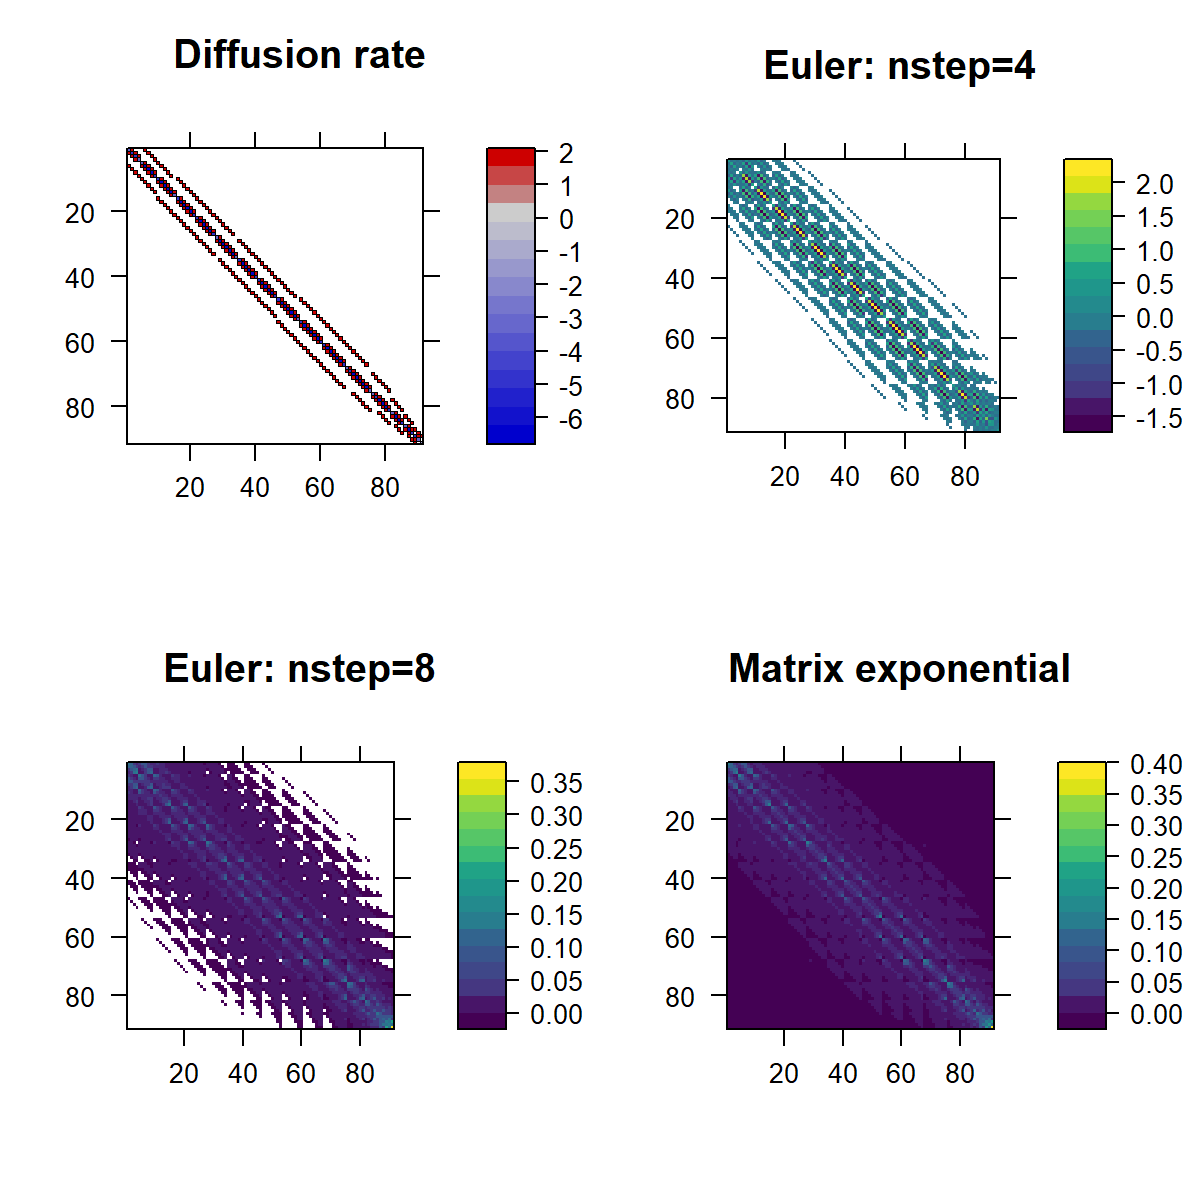
\includegraphics[width=5.5in]{Chap_10/euler_cellsize08.png}
    \label{fig:Chap10_Euler_matrices}
\end{figure}

We next extend this calculation by including movement toward preferred habitat (i.e., taxis), where we specify that habitat preference follows a lognormal distribution with optimal habitat at 100 meters above sea level.  We specifically simulate movement for 1000 individuals that are introduced on the east coast of Madagascar, using this 0.8 Latitude \(\times\) 0.8 Longitude cell size initially. This shows that individuals are initially confined to the east coast due to the presence of mountains blocking westward movement.  However, by time-interval 4 and 5, they have dispersed far enough south and north to then have viable paths to reach preferred habitat on the West Coast (Fig. \ref{fig:Chap10_movement_demo_coarse}).   

\begin{figure}[!ht]
    \caption[Projected movement for using a coarse spatial resolution]{Projected movement for 1000 individuals introduced on the east coast of Madagascar, showing elevation, habitat preference, and the stationary habitat utilization as well as abundance for 9 time-intervals starting at introduction, using a coarse-scale discretization using 0.8 latitude by 0.8 longitude cells.}
    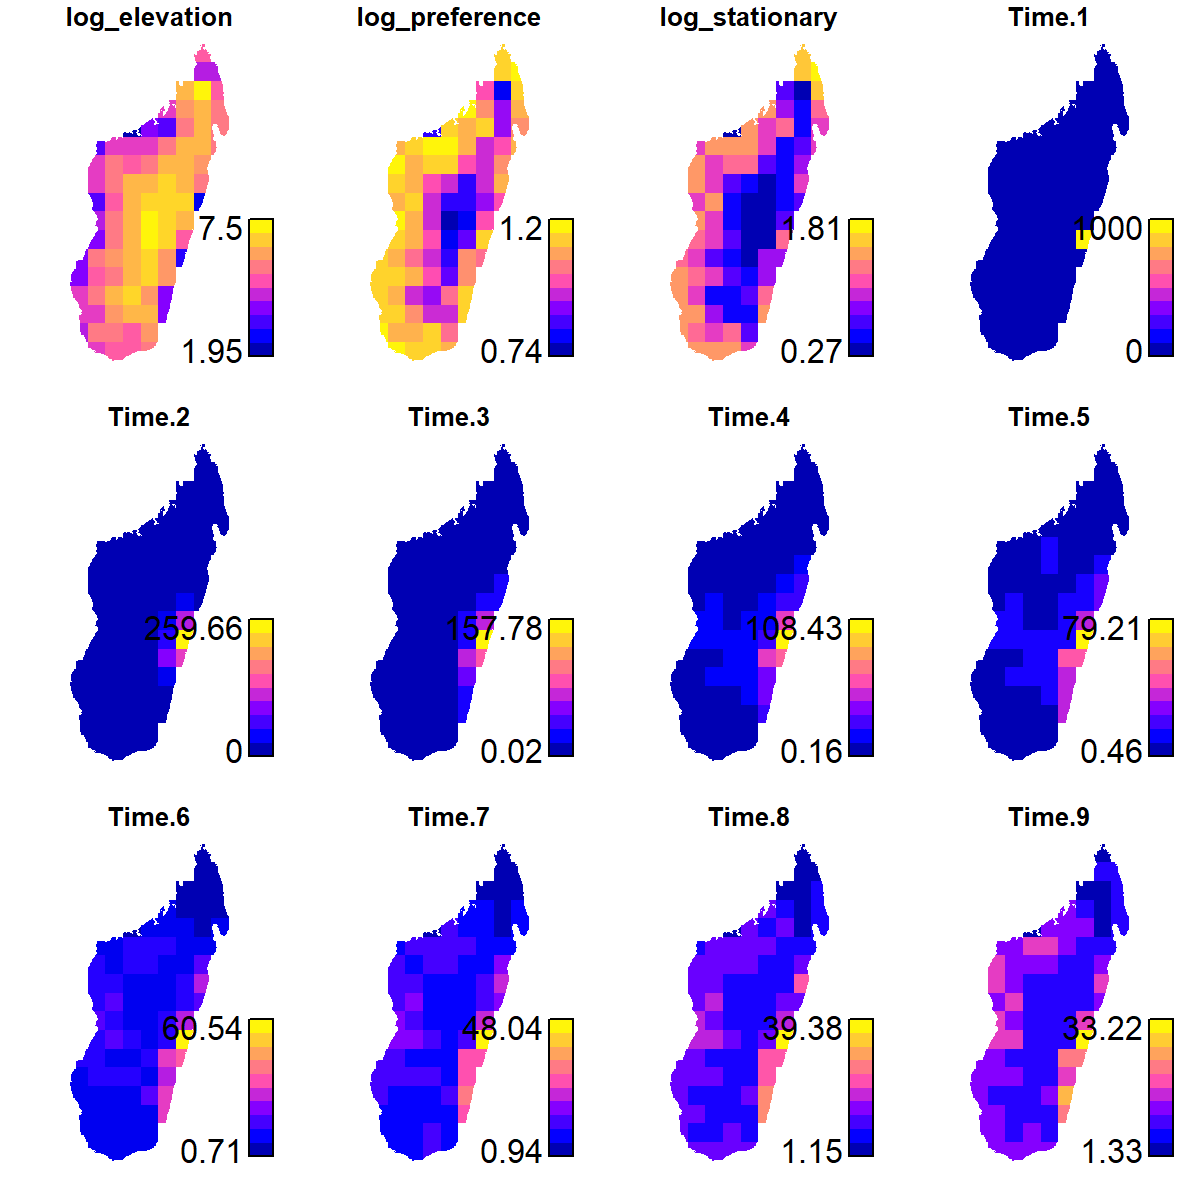
\includegraphics[width=5.5in]{Chap_10/Demo_cellsize08.png}
    \label{fig:Chap10_movement_demo_coarse}
\end{figure}

For comparison, we also illustrate the same results using 16 times more cells (i.e., a 0.2 \(\times\)0.2 cell size).  This high-resolution discretization results in a similar estimate of long-term habitat utilization. It also results in animals colonizing preferred habitats on the west coast by the 4th-5th time-interval (Fig. \ref{fig:Chap10_movement_demo_fine}).  We therefore conclude that the parameters have approximately similar interpretation regardless of the spatial scale used for discretization.   

\begin{figure}[!ht]
    \caption[Projected movement for using a fine spatial resolution]{Projected movement for 1000 individuals introduced on the east coast of Madagascar, using a fine-scale discretization using 0.2 latitude by 0.2 longitude cells (see Fig. \ref{fig:Chap10_movement_demo_coarse} for more details).}
    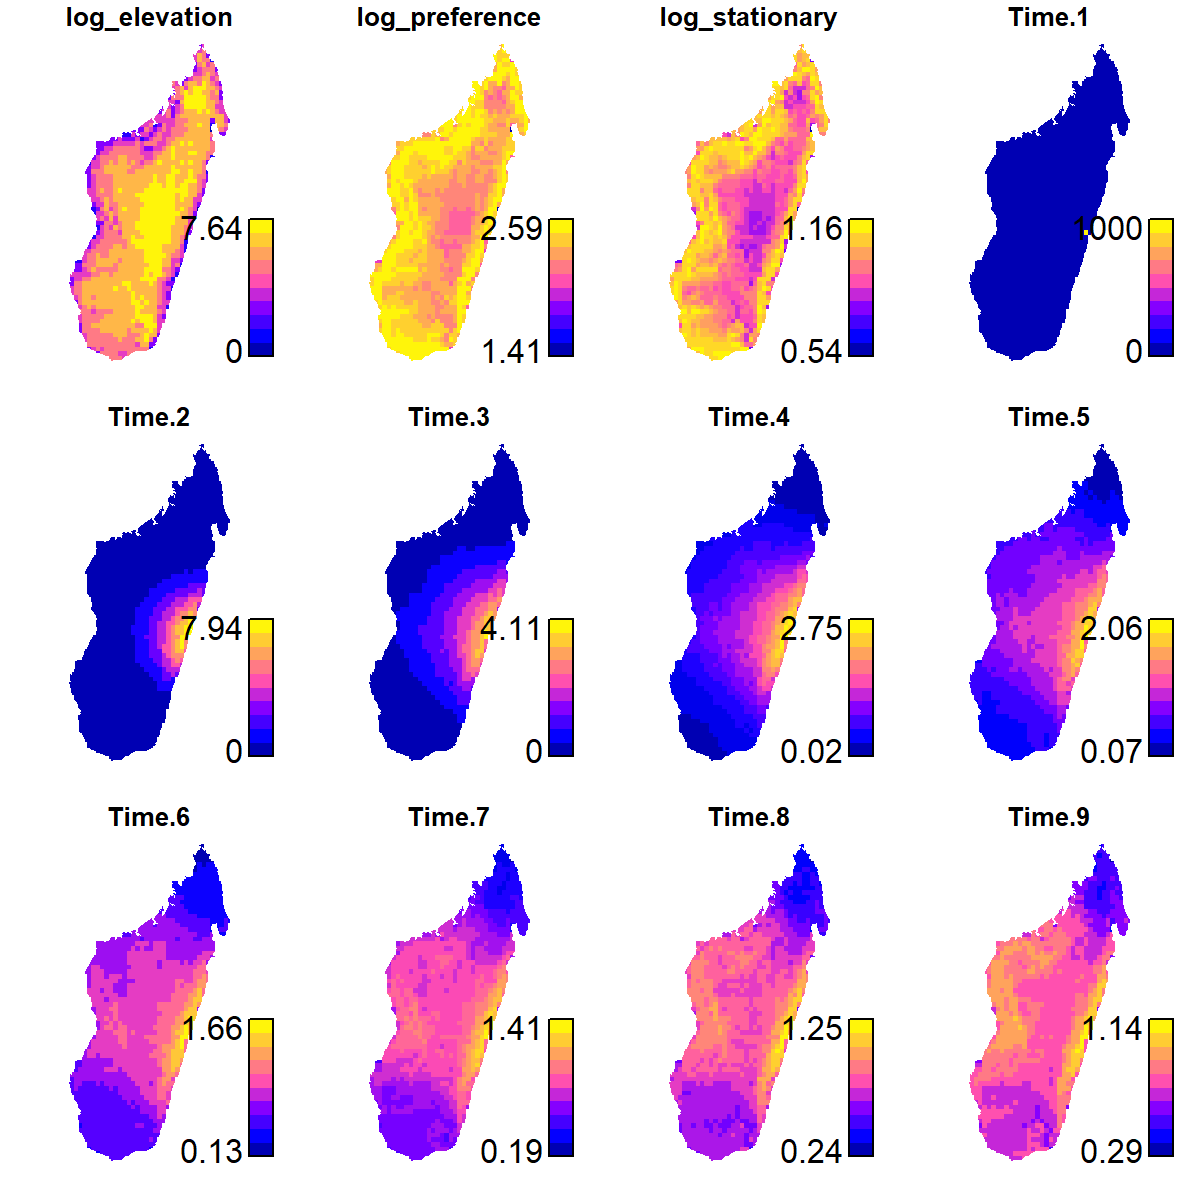
\includegraphics[width=5.5in]{Chap_10/Demo_cellsize02.png}
    \label{fig:Chap10_movement_demo_fine}
\end{figure}

In summary, this process for constructing movement matrix \(\mathbf{M}\) achieves all of our desired properties (Section \ref{sec:Chap10_solving_movement_process}):  
\begin{enumerate}
    \item[A] \textit{Conservation of numbers}: as long as the rows of rate matrix \(\dot{\mathbf{M}}\) sum to zero, then the rows of \(\mathbf{M}\) will sum to one.  This in turn implies that \( \sum_{j=1}^{n_j} n_{j,t} = \sum_{j=1}^{n_j} n_{j,t+\Delta_t} \), i.e., that movement does not change abundance; 

    \item[B] \textit{Habitat utilization as stationary distribution}:  given that movement probabilities \(\mathbf{M}\) conserve abundance, an eigendecomposition of \(\mathbf{M}\) will have one or more eigenvalues equal to \(1.0\), and other eigenvalues will be smaller.  The stationary distribution will then be a linear combination of the eigenvectors with an associated eigenvalue of \(1.0\).  Furthermore, movement probabilities \(\mathbf{M}\) and the movement rate matrix \(\dot{\mathbf{M}}\) have the same eigenvectors.  Given that the rate matrix \(\dot{\mathbf{M}}\) is sparse, we can efficiently calculate its eigendecomposition using the \colorbox{backcolour}{igraph} package \cite{csardi_igraph_2006} even for a large number of grid cells;

    \item[C] \textit{Identical parameters using either Eulerian or Lagrangian viewpoint}: by correcting for the temporal scale \(\Delta_t\) and spatial scale \(\Delta_s\) of discretization, we ensure that the Eq. \ref{eq:Chap10_PDE} is represented using the same parameters using both viewpoints;
    
    \item[D] \textit{Complicated dynamics using few parameters}:  using a linear model to assemble the habitat-preference function from covariates ensures that we can specify taxis to describe complicated movement dynamics using few parameters.  For example, we could use a polynomial or spline basis expansion to add degrees of freedom when calculating habitat preference (see Section \ref{sec:Chap5:splines});
    
    \item[E] \textit{Computational efficiency}:  finally, we can achieve computation efficiency by carefully choosing either the matrix exponential or Euler approximation, where the Euler approximation will likely be faster when a large number of grid cells are specified;

    \item[F] \textit{Scale-free discretization}:  as shown by comparing Figs. \ref{fig:Chap10_movement_demo_coarse} and \ref{fig:Chap10_movement_demo_fine}, the results are similar across a wide range of scales used for spatial discretization; 

    \item[F] \textit{Subdivision in time}: given that we project between two times \( \mathbf{n}_{t+\Delta_t}^T = \mathbf{n}_t^T e^{\Delta_t \dot{\mathbf{M}}} \), we can compute expected abundance at any intervening time as some fraction, e.g., \( \mathbf{n}_{t+0.5\Delta_t}^T = \mathbf{n}_t^T e^{0.5\Delta_t \dot{\mathbf{M}}} \) for computing the expected density at the midpoint of interval \(\Delta_t\).
\end{enumerate}
Given this general process for constructing movement matrix \(\mathbf{M}\), we next show how we can use this process to estimate movement parameters from an Eulerian viewpoint.

\section{Fitting Diffusion-taxis Movement to Individual Tracks} \label{sec:Chap10_CTMC_cod}

We first demonstrate the process of fitting this discretized movement model using an archival tag for a single tagged fish.  We previously fitted similar data in continuous space from a Lagrangian viewpoint (Section \ref{sec:Chap4_track_reconstruction}) as a state-space model.  However, this previous state-space model assumed that locations were measured following a normal distribution (Eq. \ref{eq:Chap4_measurement_distribution}), which then results in a close-to-normal distribution for random effects that can be approximately well using the Laplace approximation (recalling Section \ref{sec:Chap2_Laplace}).  By contrast, archival tags for fishes result in a distribution for measurement errors that is very different from a normal distribution (or any low-dimensional function).  We therefore use an Eulerian viewpoint to represent the measurement process more precisely.    

We specifically analyze data for a Pacific cod (\textit{Gadus macrocephalus}) that was tagged with a pop-up satellite archival tag on Feb. 21, 2019, in the Aleutian Islands \cite{bryan_seasonal_2021}. The satellite tag continuously recorded depth, temperature, and light-level data while attached to the fish.  On May 23, 2019, the tag was programmed to release from the fish and subsequently floated to the water surface where it transmitted its archived data via the ARGOS satellite network. Locations of the tagged fish were known at the time of release (using a Global Positioning System measurement) and at the time the tag began transmitting data at the water surface (provided by ARGOS). The data transmitted by the tag was used to determine the likelihood that the tagged fish occupied any given location within a specified spatial domain (Fig. \ref{fig:Chap10_data_likelihood}). The daily likelihood was calculated based on estimated longitude (derived from the time of local noon provided by light-level data) and matching the daily maximum depth of the tagged fish to bathymetric maps \cite{nielsen_geolocation_2023}\footnote{Data were collected by the Groundfish Assessment Program, Alaska Fisheries Science Center, in an effort led by Susanne McDermott. Data likelihood and covariate data were formatted, obtained, and are reproduced with permission from Julie Nielsen on Dec. 5, 2022.}.

\begin{figure}[!ht]
    \caption[Data likelihood for tagged cod]{Data likelihood \( p_{g,t} \) for evenly spaced intervals \(t\) between a Feb. 21 release and May 23 recovery for the tagged Pacific cod (panels, where white areas show land that has a zero likelihood a priori), obtained by comparing sub-daily vertical profile for the tagged individual with known bathymetry maps.}
    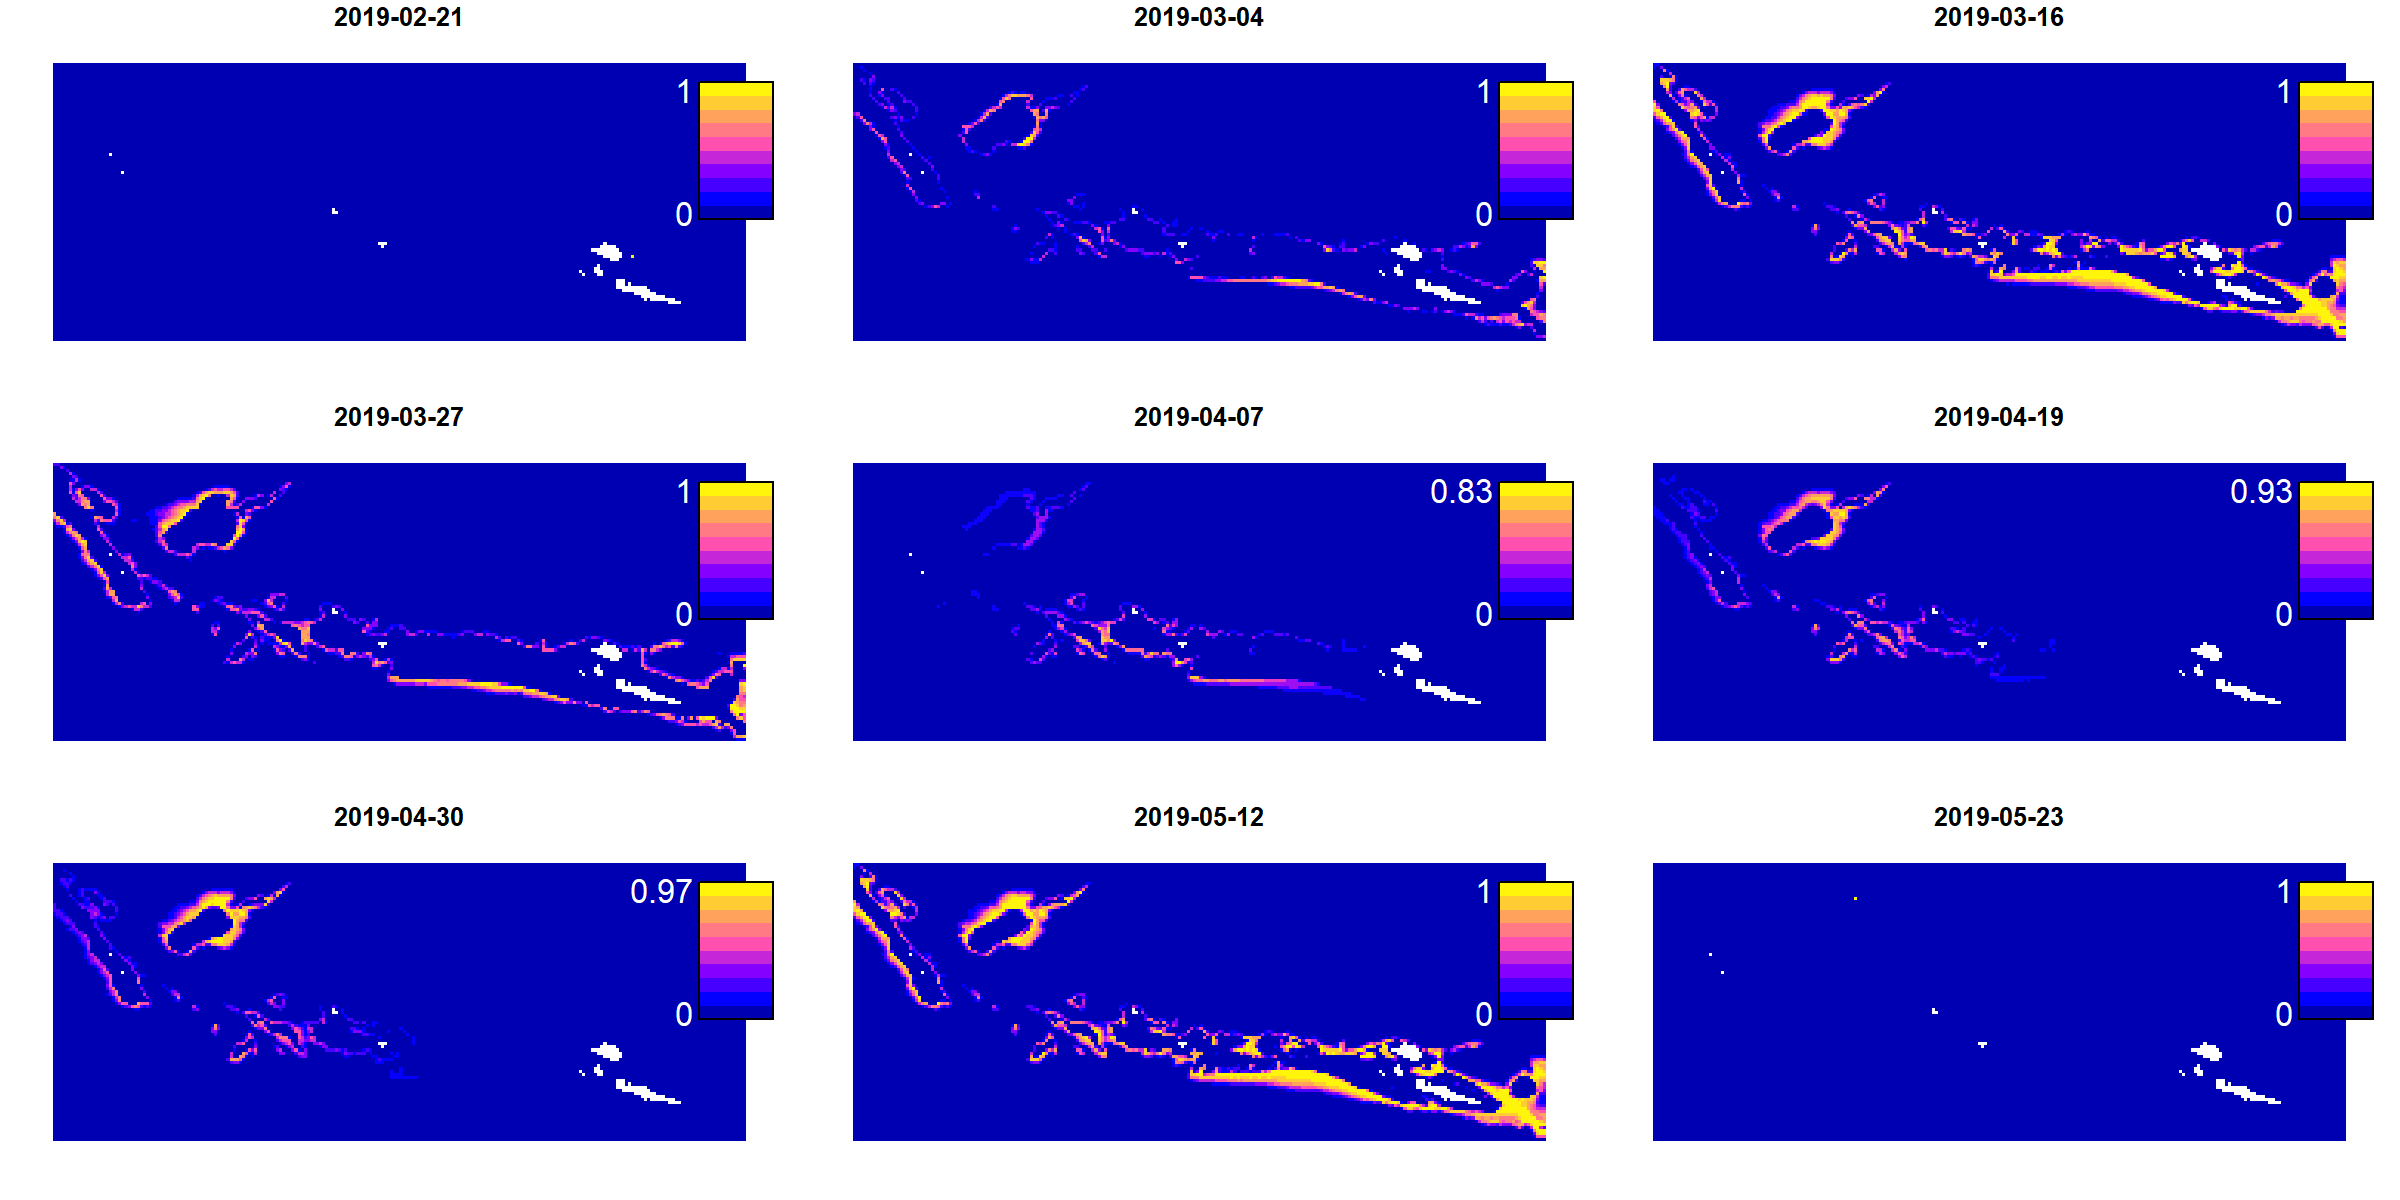
\includegraphics[width=5.5in]{Chap_10/Data_likelihood_3.png}
    \label{fig:Chap10_data_likelihood}
\end{figure}

We therefore seek to use a known location on Feb. 21 and May 23, combined with this data likelihood for location at each day between these to infer movement parameters for winter-to-spring movement of Pacific cod in the Aleutian Islands.  For this demonstration, we  define a spatial domain composed of \( 90 \times 224 = 20160 \) square grid cells, and define a daily probability \( \pi_{g,t} \) that the animal is in cell \(g\) in day \(t\).  We know seafloor depth (\textit{bathymetry}) for every grid cell, and use this as covariate to define the estimated habitat preference function.  

To do so, we fit a \myindex{hidden Markov model} (HMM).  This HMM involves defining the probability \( \pi_{g,t} \) that the individual is in a given cell \(g\) in time \(t\).  This probability evolves over time based on a transition matrix \(\mathbf{M} = e^{\dot{\mathbf{M}} \Delta_t}\), which again is calculated as the matrix exponential of a movement-rate matrix \( \dot{\mathbf{M}} \) such that:

\begin{equation}
    \pi_{t+1}^T = \pi_{t}^T \mathbf{M} 
\end{equation}
To fit this model, we have a \textit{data likelihood} surface \( p_{g,t} \) for each location \(g\) obtained from the archival tag, where this data likelihood \( p_{g_{release},1}=1 \) for the known release location \( g_{release} \) in time \(t=1\) and zero elsewhere, and again has a known recapture location \( p_{g_{recapture},n_t} = 1 \) at time of recapture \( n_t \) (see \cite{pedersen_geolocation_2008} for details).  Importantly, \( \dot{\mathbf{M}} \) has dimension \(20160 \times 20160\), and it is impractical to directly compute all 400 million cells of \( \mathbf{M} \).  We therefore use a computational technique called \textit{uniformization} \cite{grassmann_transient_1977,sherlock_direct_2021} to compute \( \mathbf{\pi}_{t}^T e^{\dot{\mathbf{M}}} \) without actually computing \( \mathbf{M} \) (see Section \ref{sec:Appendix_matrix_exponential}).

To estimate parameters and predict state-variables, we apply a \myindex{forwards-backwards algorithm} that fits this hidden Markov model to the data likelihood \( p_{g,t} \).  We seek to define the likelihood \(\Like(\theta)\) of parameters \(\theta\) so that we can calculate their maximum likelihood estimator \(\hat{\theta}\), as well as the probability of a state \(X_t\) given data \(Y_t\) and estimated parameters \(\hat{\theta}\).  Recall that we outlined how to do this in Section \ref{sec:Chap2_deriving_random_effects}, and it requires marginalizing across the value of random effects.  When analyzing location in continuous space in Section \ref{sec:Chap4_track_reconstruction}, we marginalized across locations using the Laplace approximation. Here, however, we have discrete valued states, and the Laplace approximation cannot be used for discrete-valued states.  We therefore use the alternative backwards-forwards algorithm to marginalize across latent states.  To do so, we calculate:

\begin{itemize}
    \item \textit{Marginal likelihood}:  we want to calculate the marginal likelihood \(\Like(\theta)\) of parameters \(\theta\), including those describing taxis, diffusion, and drift.  To do so, we apply a forward algorithm, which calculates the probability of state \(X_t\) for any time \(t\) given all data prior to and including that time:

    \begin{equation}
    \begin{gathered}
        \mathbf{f}_{t}^T = 
        \begin{cases}
            \mathbf{p}_{t} & \text{if } t = 1  \\
            \mathbf{p}_{t} \odot \mathbf{f}_{t-1}^T \mathbf{M}  & \text{if } t > 1  
        \end{cases}
    \end{gathered}     
    \end{equation}
    where \( \odot \) is the elementwise product of data likelihood \( \mathbf{p}_{t} \) and projected states \( \mathbf{f}_{t-1}^T \mathbf{M} \). The marginal likelihood is then calculated in the final time-interval by marginalizing across the location in that time:
    
    \begin{equation}
        \Like(\theta) = \sum_{g=1}^{n_g} \mathbf{f}_{g,n_t}        
    \end{equation}
    The log-likelihood is then maximized with respect to parameters \( \theta \) to identify preference and diffusion rates;  

    \item \textit{State probabilities}:  we also want to calculate the probability for each state given all data.  However, the quantity \( \mathbf{f}_t \) calculated by the forward algorithm for time \(t\) does not include any information from the data likelihood \(\mathbf{p}_{t^*}\) for later intervals \( t^* > t\).  To calculate the state-probability \( \mathbf{\pi}_t \) that includes all information, we repeat the same algorithm but now proceeding backwards in time.  In a lose sense, we are decomposing the data for each time into those before and including time \(t\) and those after time \(t\), where the forward algorithm calculates the former and the backwards algorithm calculates the latter:
    
    \begin{equation}
        \Pr(X_t|\text{All data}) = \Pr(X_t,\text{Past or current data}) \Pr(\text{Future data}|X_t) \propto \mathbf{f}_t \mathbf{b}_t
    \end{equation}

    This backwards algorithm involves projecting the state-probability \( \mathbf{b}_{t} \) backwards from recovery \(t=n_t\) to release time \(t=1\), while again calculating its product with the data-likelihood in each interval:

    \begin{equation}
    \begin{gathered}
        \mathbf{b}_{t} = 
        \begin{cases}
            \mathbf{1}  & \text{if } t = n_t \\  
            \mathbf{M} (\mathbf{p}_{t+1} \odot \mathbf{b}_{t+1})  & \text{if } t < n_t   
        \end{cases}
    \end{gathered}     
    \end{equation}
    We emphasize that we have defined the movement-rate matrix \( \dot{\mathbf{M}} \) such that forward-projection involves \textit{post-multiplying} the state-probability with the movement matrix \( \mathbf{f}_{t} = \mathbf{f}_{t-1}^T \mathbf{M} \), while backwards-projection involves \textit{pre-multiplying} the state probability with the movement matrix \( \mathbf{b}_{t} = \mathbf{M} \mathbf{b}_{t+1} \).  We then calculate the smoothed state-probability as the normalized product of forwards and backwards values:
    
    \begin{equation}
        \pi_{g,t} = \frac{f_{g,t} b_{g,t}}{\sum_{g'=1}^{n_g} f_{g',t} b_{g',t} }
    \end{equation}
    where this state-probability then incorporates all data as well as the estimated parameters that are represented in movement-rate \( \dot{\mathbf{M}} \).  
\end{itemize}

However, model exploration also suggested that covariates often resulted in a movement rate \( \dot{\mathbf{M}} \) that was not Metzler, i.e., where taxis was stronger than diffusion resulting in negative off-diagonal elements.  To address this, we therefore  reparameterize the instantaneous movement rate to ensure that it has  positive offdiagonal elements for any set of diffusion and taxis parameters \cite{hanks_continuous-time_2015}:   

\begin{equation}
\begin{gathered} \label{eq:Chap10_taxis2}
  \dot{m_{g_1,g_2}} = 
  \begin{cases}
    a_{g_1,g_2} \frac{D}{\Delta_s^2} e^{\frac{h_{g_2} - h_{g_1}}{\Delta_s}} & \text{if } g_1 \neq g_2  \\ 
    -\sum_{g \neq g_2} \dot{m_{g_1,g}} & \text{if } g_1 = g_2 
  \end{cases}
\end{gathered}
\end{equation}
This essentially involves the same off-diagonal calculations, but done in log-space such that their exponentiated values are always positive.  These two alternative forms for assembling movement-rates can both be implemented using sparse matrices in TMB (Code \ref{code:Chap10-assembling-movement-rate}).

\lstset{style=TMBcode}
\lstinputlisting[language=c++, label=code:Chap10-assembling-movement-rate, caption=TMB code for assembling the instantaneous movement-rate matrix., captionpos=t]{Chap_10/make_M.hpp} 

\begin{figure}[!ht]
    \caption[Pacific cod preference based on bathymetry]{Habitat preference (y-axis) estimated as a quadratic function of seafloor depth (x-axis) based on an archival tag attached to a Pacific cod in the Aleutian Islands Feb. 21 and recovered May 23, 2019, showing estimates at the original 3km grid resolution (left panel) or a coarsened 6km grid resolution (right panel) visulized using the packages \colorbox{backcolour}{marginaleffects} and \colorbox{backcolour}{ggplot2} (Section \ref{sec:Chap1_evaluating_model_fit}).}
\begin{minipage}[a]{0.5\textwidth}
    $\vcenter{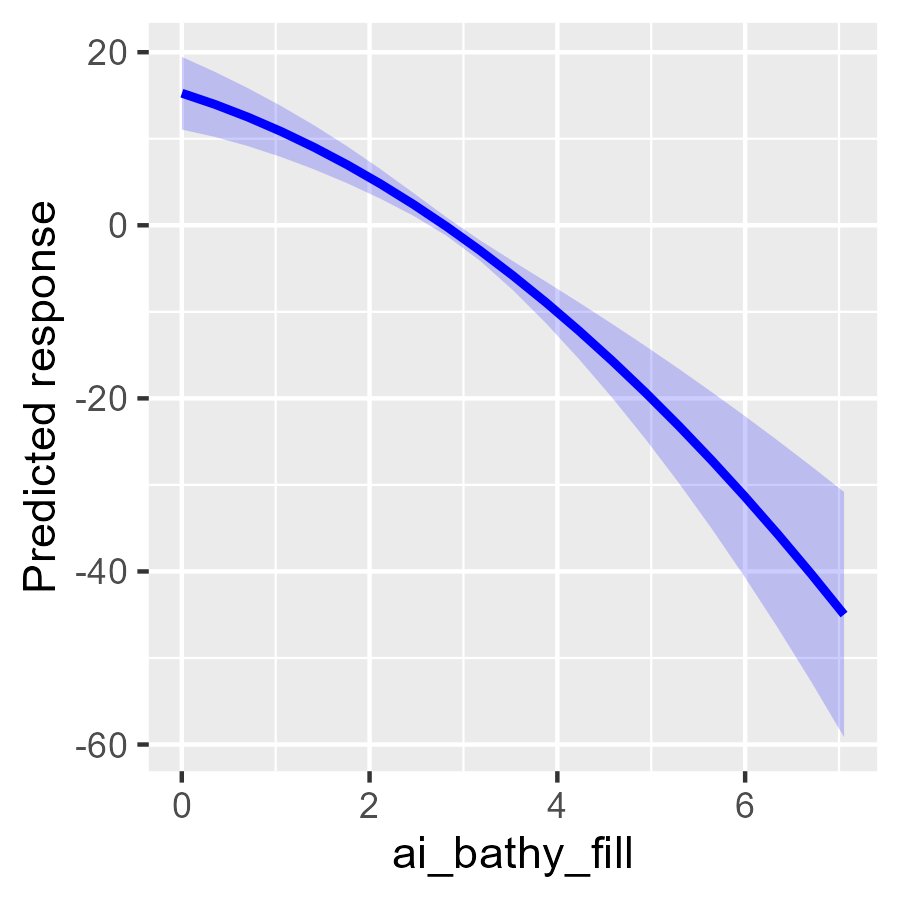
\includegraphics[width=2.75in]{Chap_10/covariate_response_3.png}}$
\end{minipage}
\begin{minipage}[b]{0.5\textwidth}
    $\vcenter{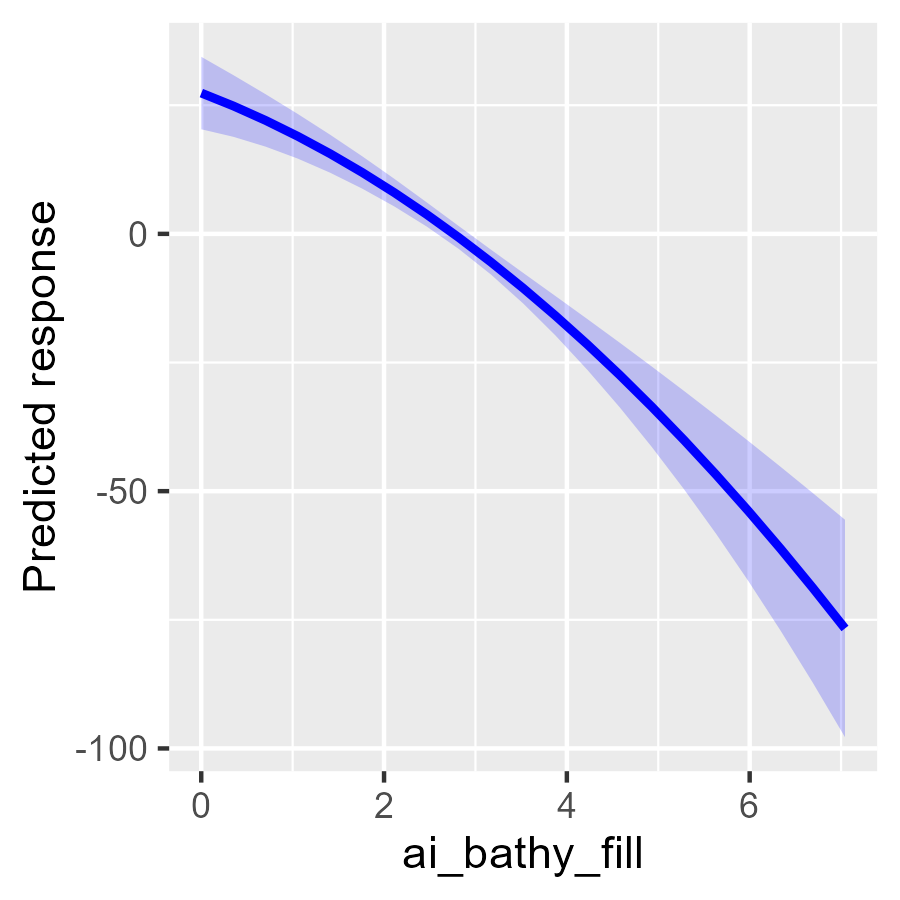
\includegraphics[width=2.75in]{Chap_10/covariate_response_6.png}}$
\end{minipage}
    \label{fig:Chap10_cod_covariate}
\end{figure}

We fit this model by maximizing the marginal likelihood in R.  The latent states are integrated using the forwards-backwards algorithm and we do not specify any additional random effects, so the model is implemented using TMB without applying the Laplace approximation.  We specify the habitat preference \( h_g  = \gamma_1 x_g + \gamma_2 x_g^2 \) as a quadratic function of bathymetry \(x_g\), and the estimated response function suggests a strong preference for shallow depths (Fig. \ref{fig:Chap10_cod_covariate}).  We can also visualize the estimated preference function on a map (Fig. \ref{fig:Chap10_cod_results}).  The map of bathymetry shows relatively shallow depths running along a band southeast to northwest, and Pacific cod clearly prefer this shallow band.  Calculating habitat utilization as the stationary distribution (i.e., the eigendecomposition of \(\dot{\mathbf{M}}\)) indicates that this individual cod is expected to reside in larger discrete patches of preferred habitat, and therefore likely uses corridors of preferred habitats to rapidly cross from patch to patch.     

\begin{figure}[!ht]
    \caption[Pacific cod habitat preference and distribution at 3 km resolution]{Bathymetry (top row), estimated habitat preference (middle row) and resulting stationary distribution (bottom row) based on fitting to an archival tag for Pacific cod at the original 3km grid resolution (left column) or a coarsened 6km grid resolution (right column).  Note that areas with bathymetry less than 1 m are excluded (white areas in each map).}
\begin{minipage}[a]{0.5\textwidth}
    $\vcenter{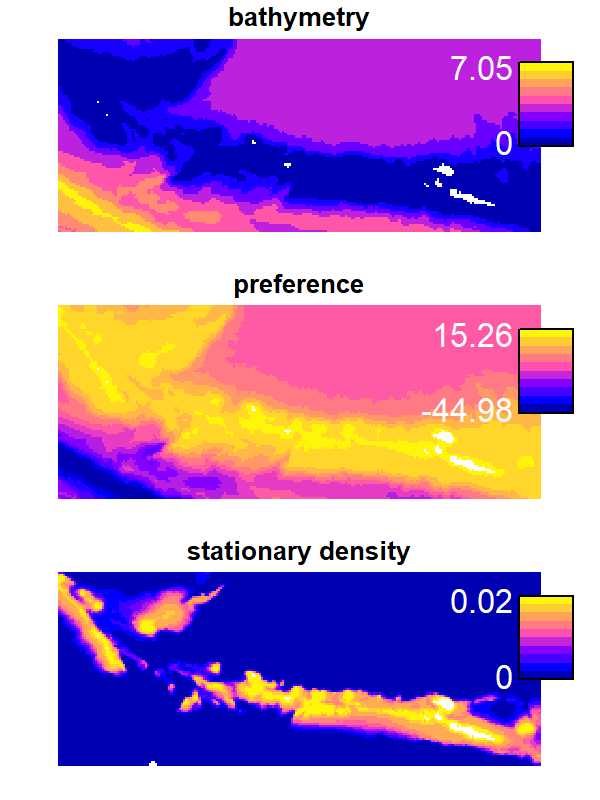
\includegraphics[width=2.75in]{Chap_10/Small_results_3.png}}$
\end{minipage}
\begin{minipage}[b]{0.5\textwidth}
    $\vcenter{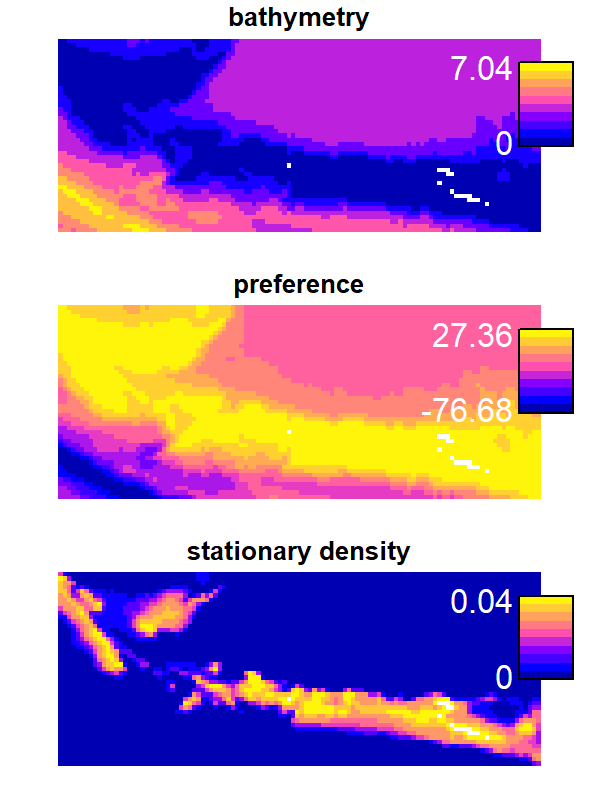
\includegraphics[width=2.75in]{Chap_10/Small_results_6.png}}$
\end{minipage}
    \label{fig:Chap10_cod_results}
\end{figure}

Finally, the smoothed state-probabilities \( \pi_{g,t} \) show that the animal released on Feb. 21 in the southeastern portion of the modeled domain likely moved west until early April, when it then made a rapid movement north toward the northern boundary (Fig. \ref{fig:Smoothed_cod_results}).  It then likely resided in that northern area through the remainder of the tagged period.   

\begin{figure}[!ht]
    \caption[Smoothed state-probabilities for tagged cod]{Smoothed state probabilities \( \pi_{g,t} \) for evenly spaced intervals \(t\) between a Feb. 21 release and May 23 recovery for the tagged Pacific cod, estimated using 3 km \(\times\) 3 km resolution but noting that 6km resolution results are similar.}
\centering
    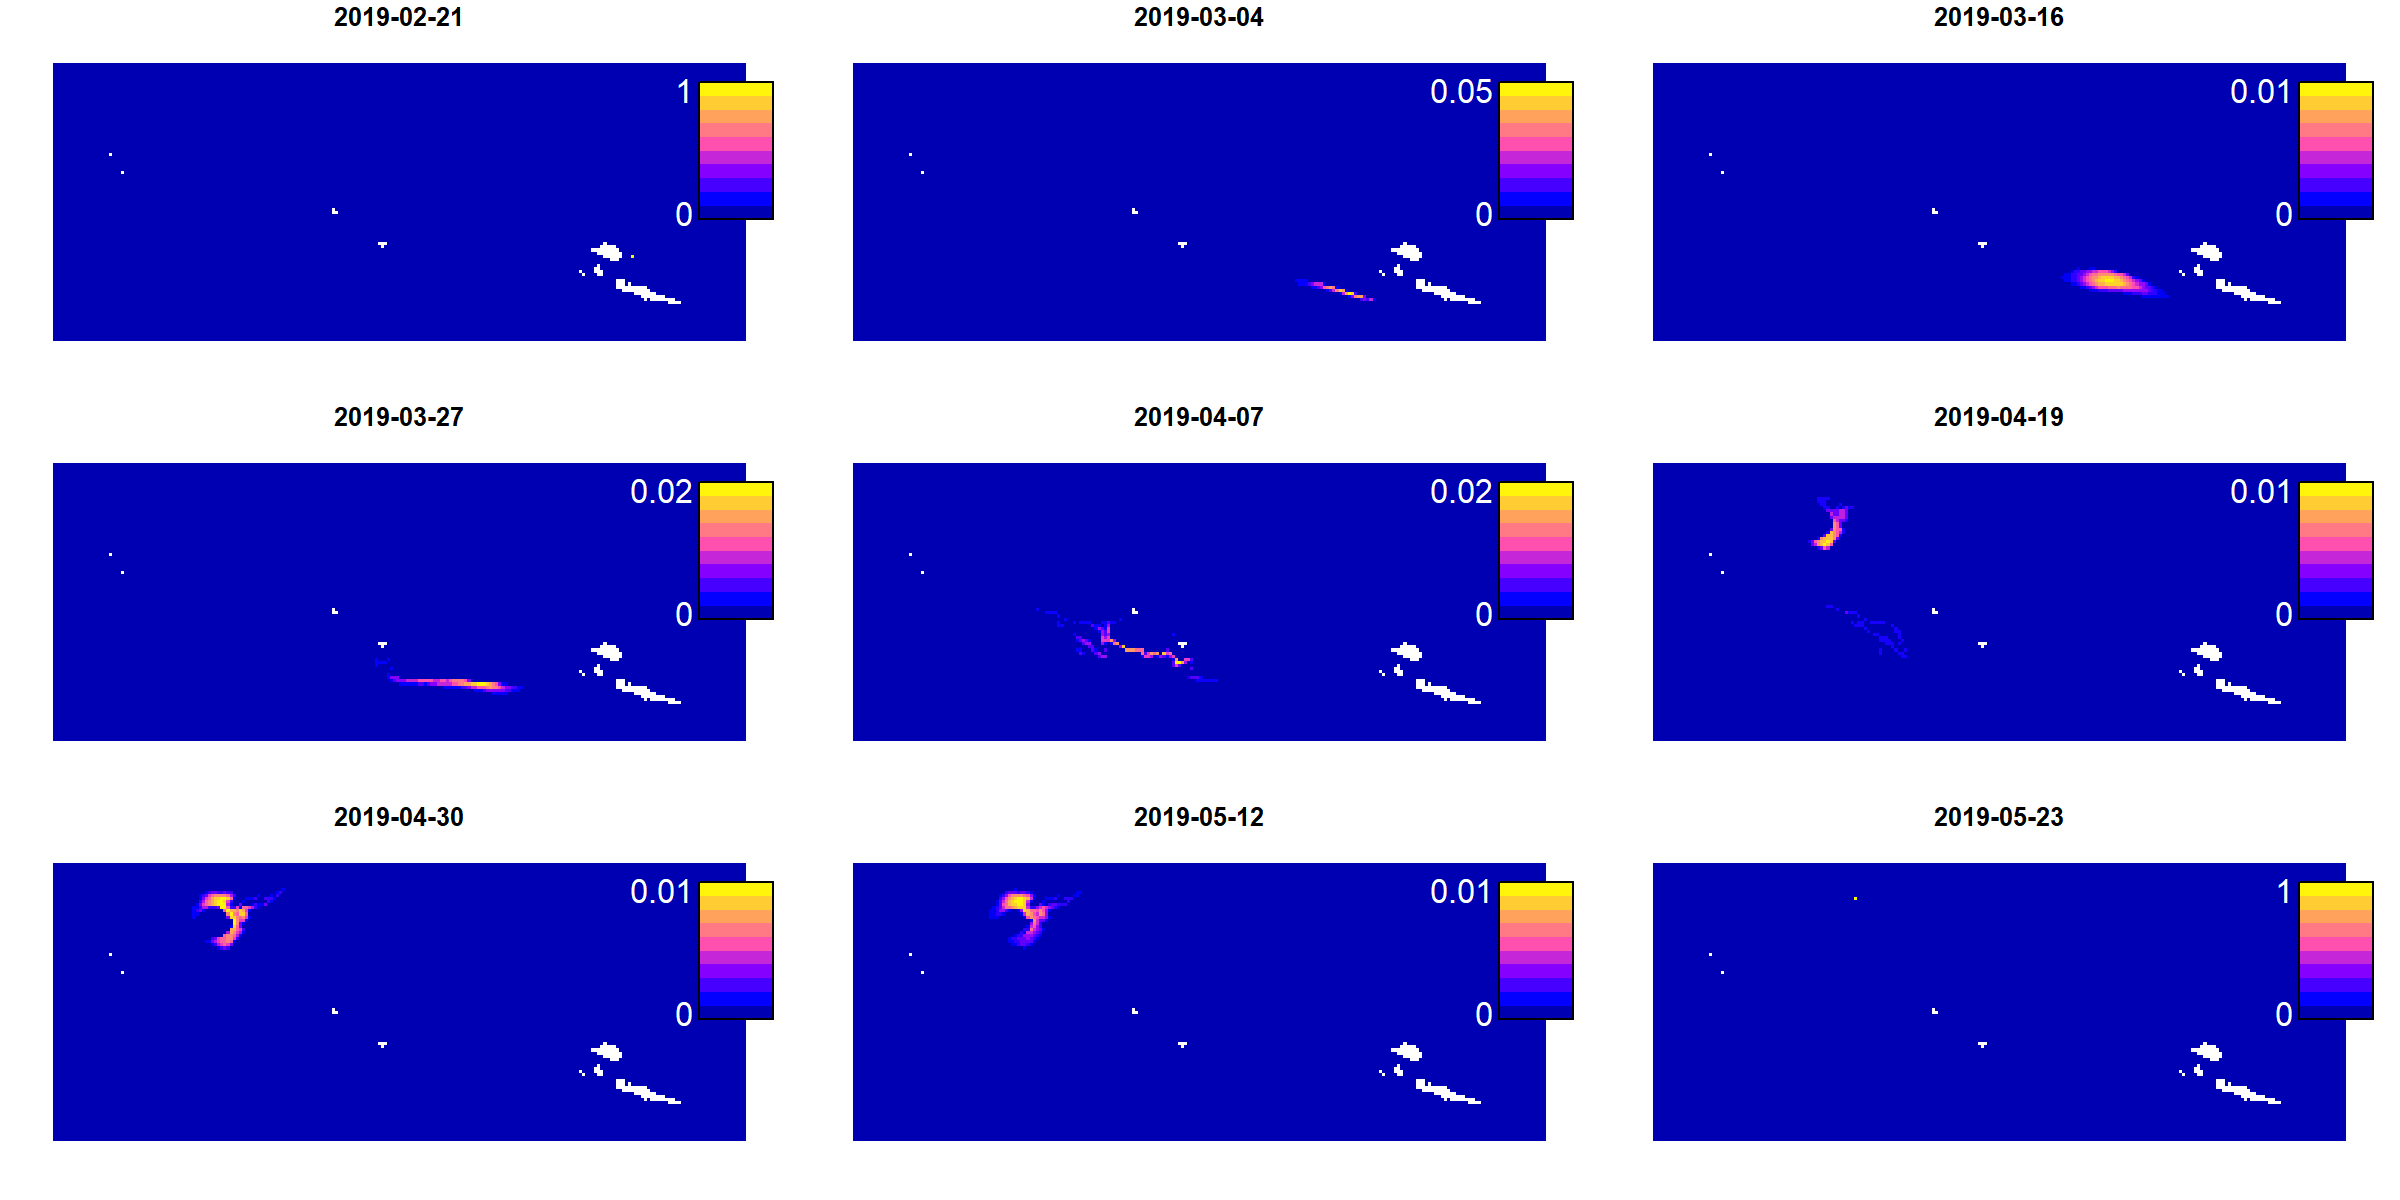
\includegraphics[width=5.5in]{Chap_10/Smoothed_results_3_Small.png}
    \label{fig:Smoothed_cod_results}
\end{figure}

\section{Fitting Diffusion-taxis Movement to Point-count Data} \label{sec:Chap10_CTMC_eagle}

So far, we have demonstrated how to fit a movement model to location measurements for a single individual, using either a state-space model from a Lagrangian viewpoint (Section \ref{sec:Chap4_track_reconstruction}) or a Hidden Markov Model from an Eulerian viewpoint (Section \ref{sec:Chap10_CTMC_cod}).  The Eulerian viewpoint seems particularly appropriate when the measurement likelihood is highly non-normal, but otherwise, the two can be constructed to fit the same underlying process (Eq. \ref{eq:Chap10_PDE}).  

However, the Eulerian viewpoint has important advantages when fitting a movement process to point-count data such as those we analyzed from Chapter \ref{sec:Chap5} onwards.  We specifically explore a scenario where density is measured but tagging data are not available.  We therefore use movement rates to inform changes in population density over time, similar to what is often done in species distribution/density models.  Past studies have used a similar model to project population range expansion for invasive species \cite{hooten_statistical_2010}, or to fit an integrated model that includes both density samples and tagging data \cite{thorson_estimating_2021}.

\begin{figure}[!ht]
    \caption[Sparsity pattern for bald eagle movement model]{Sparsity pattern for random effects in a model for eagle movement 1966--2019, where densities are block-tridiagonal because density \( \mathrm{log}(d_{g,t-1}) \) is conditionally independent of \( \mathrm{log}(d_{g,t+1}) \).}
\centering
    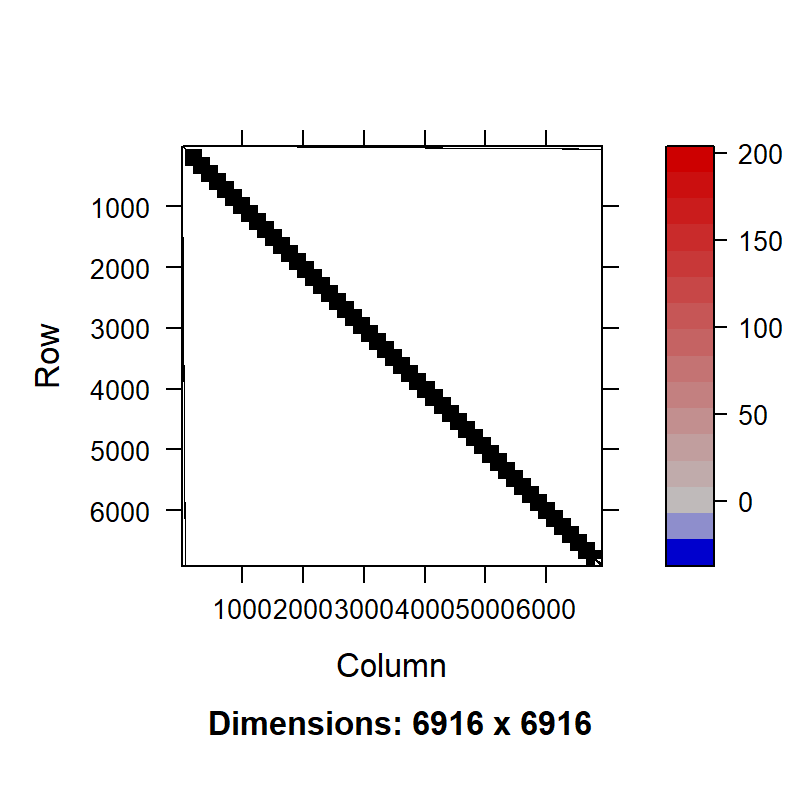
\includegraphics[width=4in]{Chap_10/Eagle_sparsity.png}
    \label{fig:Chap10_eagle_sparsity}
\end{figure}

We specifically revisit the bald eagle data set from Chapter \ref{sec:Chap5}, but now analyzing spatio-temporal data from 1968--2019 and from Alaska to California.  We specifically seek to explore drivers for population range expansion as its population recovered following a ban on DDT \cite{eakle_wintering_2015}.  Following the steps in Section \ref{sec:Chap10_solving_movement_process}, we first discretize the spatial domain into 93 square grid cells (each 250 km by 250 km), and calculate the rook-move adjacency matrix.  We then obtain elevation, satellite measurements of green vegetation (the Normalized Difference Vegetation Index or \textit{NDVI}), and distance to coastline as covariates, and model preference as a quadratic function of each covariate (i.e., 6 preference parameters total).  We use these covariates to define the movement rate \(\dot{\mathbf{M}}\) and integrate movement matrix \(\mathbf{M}\).    

We then treat \( \log(d_{g,t}) \) as a random effect while specifying:

\begin{equation}
\begin{gathered} \label{eq:Chap10_eagles}
  \hat{\mathbf{d}}_{t} = 
  \begin{cases}
    e^{\beta_1} \times \mathbf{1} & \text{if } t=1  \\ 
    e^{\beta_t} \times \mathbf{d}_{t-1}^T e^{\dot{\mathbf{M}}} & \text{if } t>1   
  \end{cases} \\ 
  \log(\mathbf{d}_{t}) \sim \mathrm{MVN} \left( \log(\hat{\mathbf{d}}_{t}), \mathbf{Q}^{-1} \right) 
\end{gathered}
\end{equation}
where \(\beta_1\) is the average log-abundance in the first modeled year, subsequent values \(\beta_t\) represent interannual changes in log-densities, and \( \mathbf{Q} \) is the precision matrix derived from a conditional autoregressive process (see Eq. \ref{eq:Chap5_CAR}).  Importantly, we specify the state variable \( \log(d_{g,t}) \) as random effect so that \( \log(d_{g,t-1}) \) is independent of \( \log(d_{g,t+1}) \) conditional upon the fixed value of \( \log(d_{g,t}) \).  This then results in a sparse inner Hessian for log-density \( \log(\mathbf{D}) \) (recalling Section \ref{sec:Chap2_Hessian_sparsity}), as confirmed in Fig. \ref{fig:Chap10_eagle_sparsity}.  We specify a spatially correlated random effect in each modeled time as a series of conditional distributions (e.g., directly specifying Eq. \ref{eq:Chap8_nonseparable}).  This results in a \myindex{non-separable model}, but it clearly serves a useful role by decomposing dynamics into separate components representing changes in log-density \(\beta_t\) versus spatial distribution shifts \(\dot{\mathbf{M}}\).  

We complete the model by specifying a Poisson distribution for counts.  We are fitting point counts without any tagging data, and prior studies suggest that it is not feasible to separately estimate diffusion rates and the magnitude of habitat preferences without tagging data \cite{thorson_estimating_2021}.  We therefore choose to fix diffusion \(D\) at a fixed value.  To do so, we note that juvenile bald eagles typically disperse 80 km and the age of first reproduction is approximately 5 years, so mean-squared displacement (MSD) is \(80^2 \: km^2\) when \(\Delta_t = 5\) years.  Remembering that the mean-squared displacement \(MSD = 2nD\Delta_t\) (introduced in Eq. \ref{eq:Chap4_MSD}), we obtain \(D = \frac{80^2}{2 \times 2 \times 5} \: km^2 \cdot year^{-1}\).  

\begin{figure}[!ht]
    \caption[Habitat preference for bald eagle movement]{Habitat preference functions (y-axis) estimated as a quadratic function of elevation (left panel), Normalized Difference Vegetation Index (middle panel) or distance from coastline (right panel), and noting that the y-axis scale (and resulting magnitude of covariate effects) differs between panels, visualized using the \colorbox{backcolour}{marginaleffects} package.}
    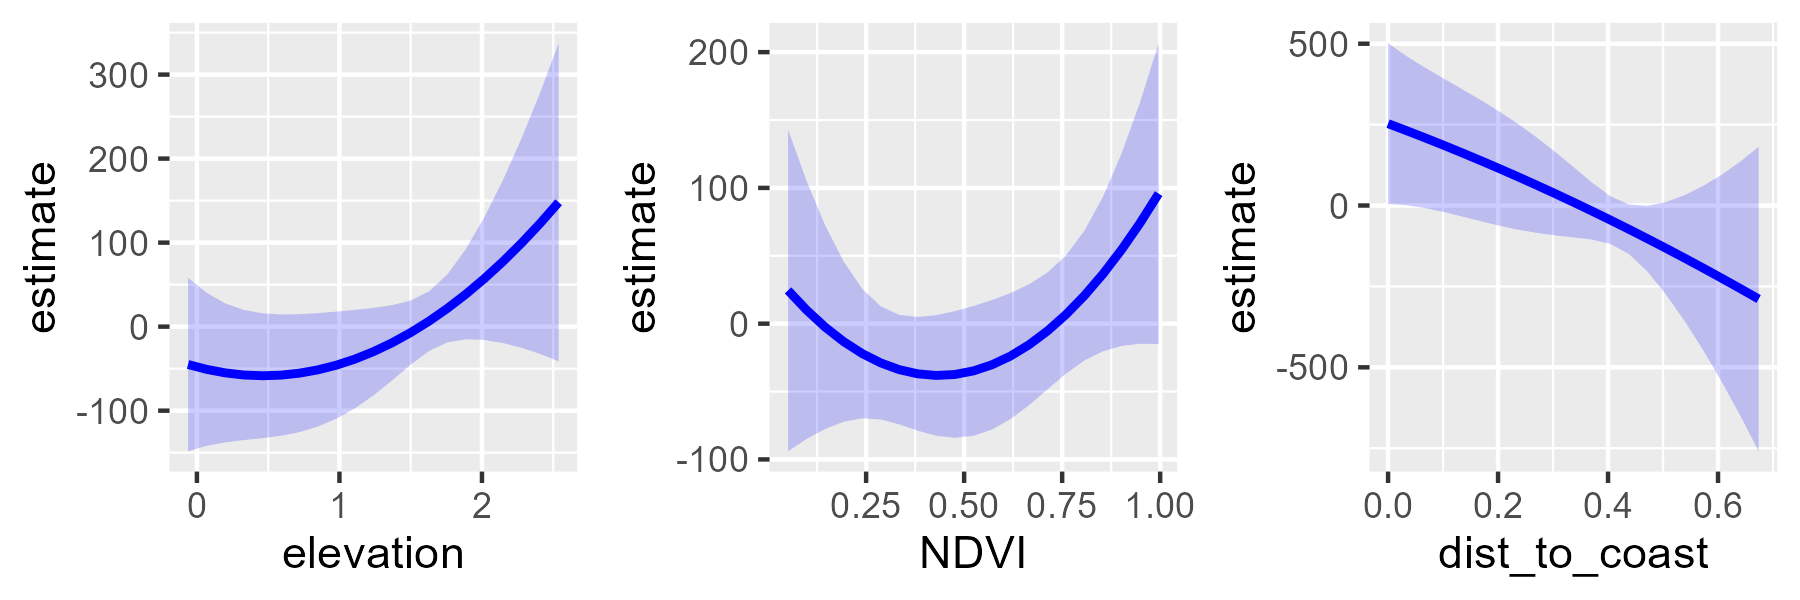
\includegraphics[width=5.5in]{Chap_10/Eagle_covariate_response.png}
    \label{fig:Chap10_eagle_covariate_response}
\end{figure}

Inspecting results, we see that bald eagles prefer habitats that are close to the coastline and higher elevation all else equal (Fig. \ref{fig:Chap10_eagle_covariate_response}). We can again map these covariates and the resulting habitat preferences (Fig. \ref{fig:Chap10_eagle_results}) and confirm that the predicted preference is lower for areas that are relatively far from the coast. Finally, inspecting estimates of density show that bald eagles had a relatively constrained distribution in Southeast Alaska and British Columbia in 1968, but recolonized habitats in Washington and Oregon by 1978 and subsequently increased in California by 2008--2019.  In particular, population density in  later years is generally proportional to the estimated preference function, suggesting that the population has recolonized most of its preferred habitat in the western portion of North America.           

\begin{figure}[!ht]
    \caption[Mapped preference and range recovery for bald eagles]{Mapped values of elevation, NDVI, and distance from coastline, the resulting prediction of habitat preference, and estimated bald eagle log-densities for evenly spaced years 1968-2019.}
    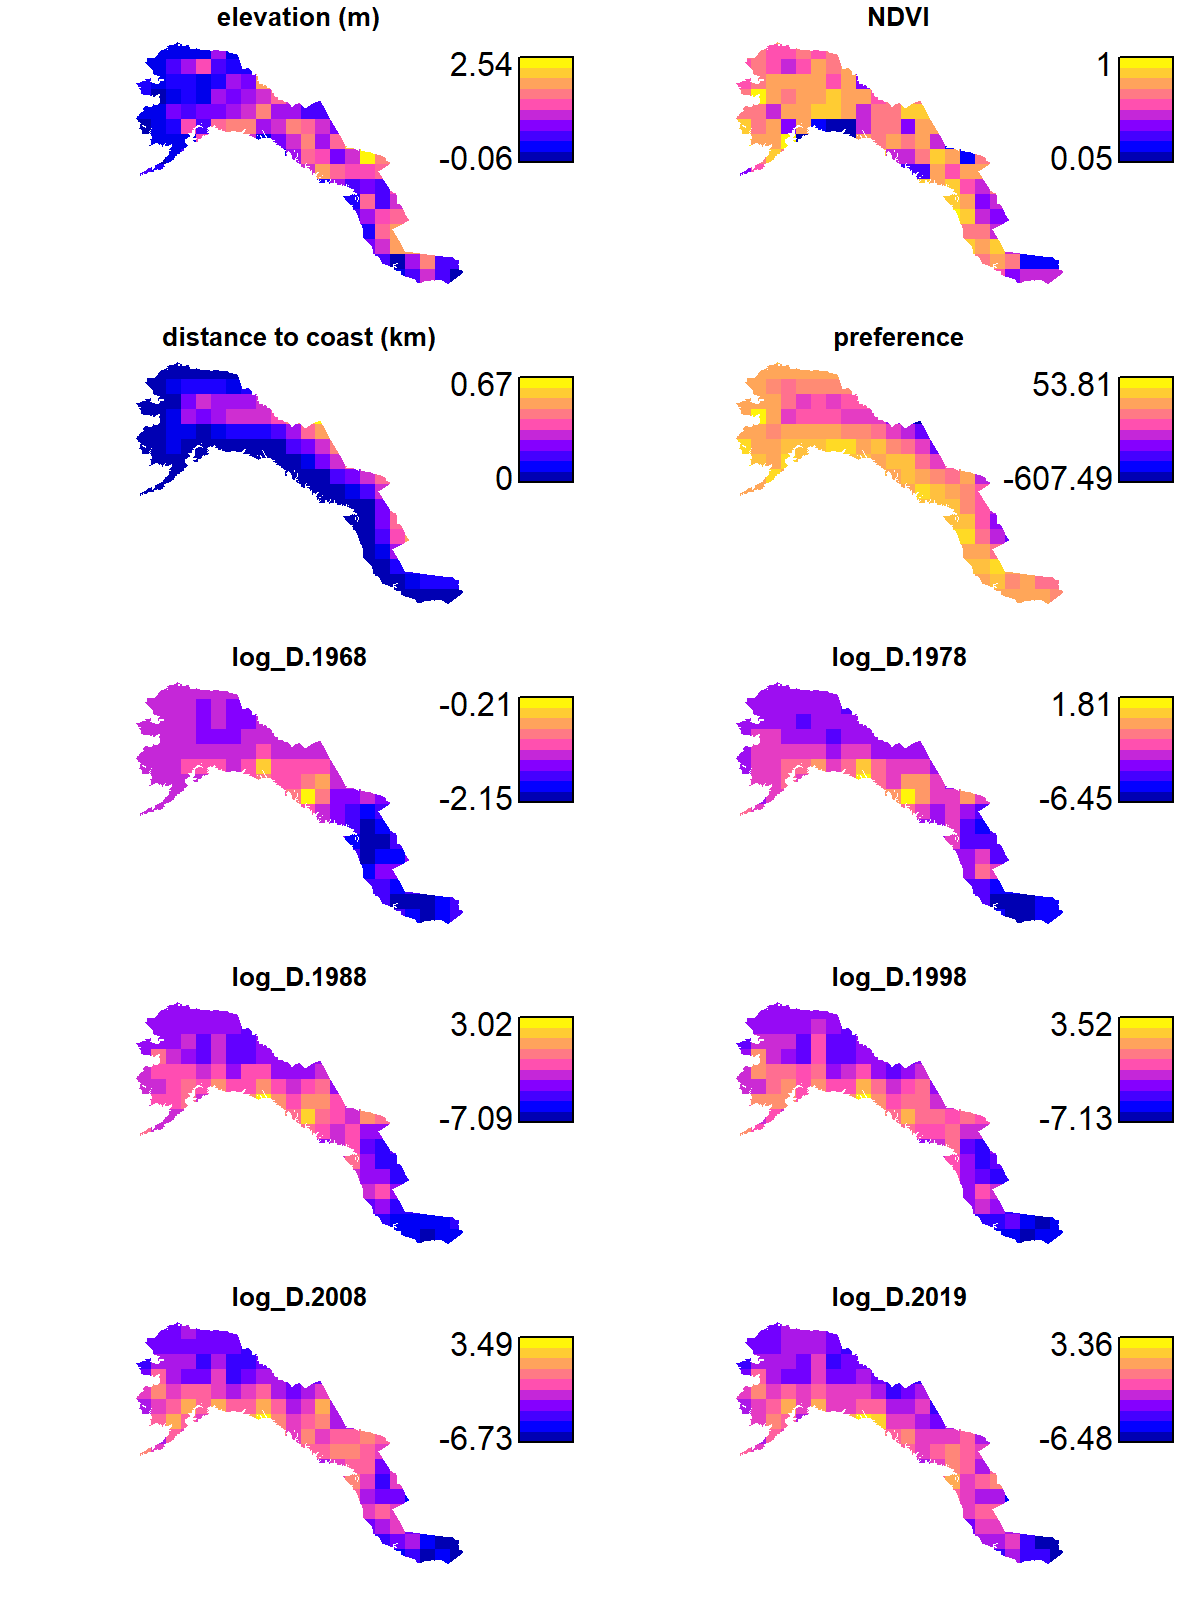
\includegraphics[width=5.5in]{Chap_10/Eagle_results.png}
    \label{fig:Chap10_eagle_results}
\end{figure}

\section{Chapter Summary}

\begin{figure}[!ht]
    \caption[Decision tree for using taxis-diffusion-drift movement model]{A simplified decision tree explaining how to use the partial differential equation that includes taxis, drift, and diffusion terms to explain movement (Eq. \ref{eq:Chap10_PDE}).  Decisions are shown in boxes, and these include identifying vector-fields for drift, covariates for the habitat preference function, rates for diffusion, and decisions about the discretization that depend upon the intended usage.}
    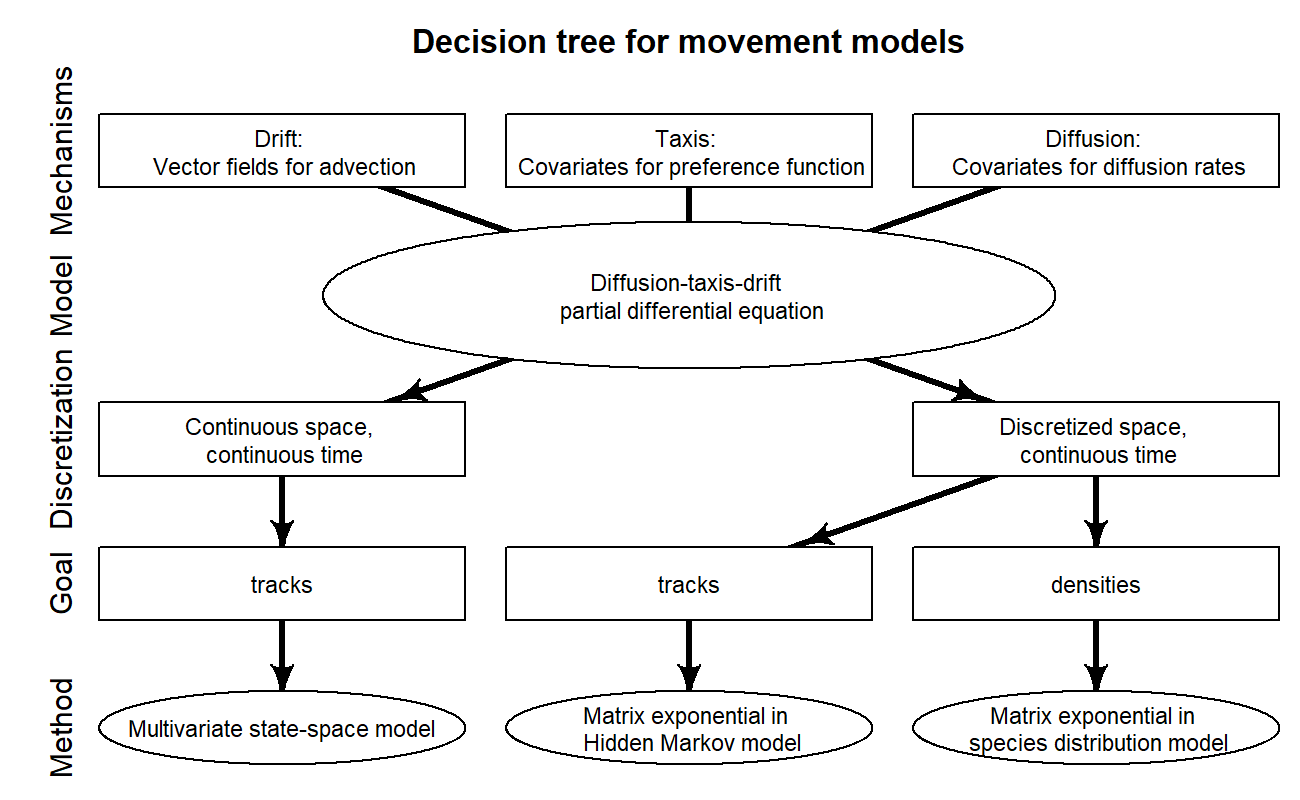
\includegraphics[width=5.5in]{Chap_10/Decision_tree_for_movement.png}
    \label{fig:Chap10_decision_tree}
\end{figure}

In summary, we have showed that:
\begin{enumerate}
    \item Individual movement can be represented using a partial differential equation that includes components for taxis, drift, and diffusion.  This process can be represented from a Lagrangian (individual-based) viewpoint using a multivariate state-space model (Chap. \ref{sec:Chap4_movement}) to estimate movement parameters and reconstruct tracks for a small set of individuals.  It can also be discretized across space and modeled from an Eulerian (grid-based) viewpoint, by defining instantaneous movement rates and then solving for movement fractions by applying a matrix exponential operator.  The movement-rate matrix can itself be constructed by adding together the effect of taxis, drift, and diffusion matrices.  When tracking the probability that a single individual is in each spatial cell, parameters can be estimated using a Hidden Markov model (HMM) forwards algorithm, and location can be subsequently estimated using both the forwards filter and backwards smoother.  Finally, the spatially discretized movement model can be applied to a vector representing population density for a population.  This density or probability vector is then projected forward in time by multiplying it with a movement-fraction matrix.  These various options are summarized in Fig. \ref{fig:Chap10_decision_tree};

    \item This matrix exponential can be calculated efficiently either by using the Euler approximation (which pre-specifies the maximum number of grid-cells that can be moved in a single time-interval), or using uniformization (which calculates the product of the density vector and matrix exponential without directly computing the latter).  Similarly, parameters can be specified without bounds if the movement-rate matrix is constructed with log-linked rates, such that directional movement from one to any other cell is guaranteed to be positive;  

    \item Using uniformization, it is feasible to estimate movement among thousands of spatial grid cells when fitting to individual animal tracks.  This procedure results in parameter estimates that are largely independent of the spatial scale used for discretizing space;   

    \item Similarly, habitat preference parameters and resulting movement can be estimated directly from point-count data by specifying the diffusion rate a priori.  This then allows spatio-temporal models to be fitted with covariates that inform habitat preferences rather than habitat-response functions in a conventional species distribution model.  This results in a non-separable model, but the inner Hessian is still sparse such that the model can be fitted efficiently to data.  
\end{enumerate}

\section{Exercises}

\begin{enumerate}
    \item In Eq. \ref{eq:Chap10_PDE}, we define the PDE for diffusion-taxis-drift movement. This includes the term \(D \nabla^2 d(s,t)\) for isotropic diffusion, and Code \ref{code:Chap10-analytical-solution} showed how to check this numerically using a diffusion-only process in R. However, the Laplacian operator can instead be generalized by writing \(D \nabla \cdot \mathbf{\Sigma} \nabla d(s,t)\), where \(\mathbf{\Sigma}\) is an \myindex{anisotropic diffusion} matrix, representing a different diffusion rate in different cardinal directions.  How specifically would you code a transformation \(\mathbf{\Sigma}\) to represent fastest diffusion in the northwest-southeast axis, and what ecological conditions might give rise to anisotropic diffusion?
    
    \item In Section \ref{sec:Chap10_CTMC_eagle}, we showed how to fit a diffusion-taxis movement model to point-count data.  This is more conventionally done using regression-based species distribution models (SDM), such as the separable model with an autocorrelated interaction of space and time introduced (Eq. \ref{eq:Chap8_spatiotemporal_AR}).  Please refit the bald eagle data using that alternative spatio-temporal model, while also adding the quadratic effect of elevation, NDVI, and distance to the coastline as density covariates.  How do the estimated covariate-response curves differ between the movement model and the regression-based SDM?   
\end{enumerate}

